%-----------------------------------------------------------------------------%
\chapter{IMPLEMENTASI DAN PENGUJIAN}
%-----------------------------------------------------------------------------%

%
\vspace{4.5pt}
\noindent Pada bab ini akan menjelaskan mengenai proses implementasi dan pengujian terhadap sistem yang telah dibangun berdasarkan penjelasan pada bab sebelumnya.\\

\section{Lingkungan Implementasi}
\noindent Pada lingkungan implementasi, akan dijelaskan mengenai perangkat yang digunakan dalam proses pembangunan sistem baik dari perangkat keras maupun perangkat lunak yang digunakan.\\

\subsection{Spesifikasi Perangkat Keras}
\noindent Spesifikasi dari perangkat keras yang digunakan dalam pembangunan aplikasi adalah sebagai berikut:
\begin{enumerate}[noitemsep]
\item \textit{Laptop} ASUS A442UQ
\item \textit{Processor} Intel Core i7-7500U CPU @ 2.7GHz
\item \textit{Hard Disk} kapasitas 1TB
\item RAM 16GB\\
\end{enumerate}

\subsection{Lingkungan Perangkat Lunak}
\noindent Spesifikasi dari perangkat lunak yang digunakan dalam pembangunan aplikasi adalah sebagai berikut:
\begin{enumerate}[noitemsep]
\item Sistem Operasi Windows 10 Home 64 bit.
\item Netbeans IDE 8.2
\item Java Development Kit (JDK) 1.8.0{\_}161
\item \textit{Library} OpenCV 3.4.6\\
\end{enumerate}

\section{Implementasi Perangkat Lunak}
\noindent Pada bab ini akan dijelaskan mengenai implementasi aplikasi untuk pengenalan karakter pada citra plat kendaraan. Di bawah ini merupakan daftar \textit{class} dan \textit{method} beserta penjelasan mengenai cara kerja program.\\
\subsection{Daftar \textit{Class} dan \textit{Method} Gradient}
\noindent Berikut adalah tabel berisi \textit{method} pada \textit{class} Gradient. \textit{Class} Gradient digunakan untuk menyimpan nilai \textit{orientation} dan nilai \textit{magnitude} dari suatu piksel citra.
\begin{small}
	\begin{longtable}{| p {0.5cm} | p {3cm} | p {4cm} | p {1.5cm} | p {3cm} |}
		\caption{Daftar \textit{Method Class Gradient} } \\
		\hline
		\textbf{No}  & \textbf{Nama \textit{method}}  & \textbf{Masukan}  & \textbf{Keluaran} & \textbf{Keterangan} \\ \hline
		\endhead	
		1	& Gradient & double orientation, double magnitude & void & Metode \textit{constructor} yang digunakan untuk inisialisasi objek dari kelas Gradient dengan nilai \textit{orientation} dan \textit{magnitude} yang didapatkan dari perhitungan. \\
		\hline
		2	& getOrientation() & & double & Metode untuk mengembalikan nilai \textit{orientation} dari suatu piksel.\\
		\hline
		3	& getMagnitude() & & double & Metode yang digunakan untuk mengembalikan nilai \textit{magnitude} dari suatu piksel.\\
		\hline
		4	& setOrientation() & double orientation & void & Metode untuk mengatur nilai \textit{orientation} dari objek Gradient berdasarkan nilai \textit{orientation} yang dijadikan masukkan.\\
		\hline
		5	& setMagnitude() & double magnitude & void & Metode yang digunakan untuk mengatur nilai \textit{magnitude} dari objek Gradient berdasarkan nilai \textit{magnitude}  yang dijadikan masukkan.\\
		\hline
	\end{longtable}
\end{small}

\subsection{Daftar \textit{Class} dan \textit{Method} GradientCell}
\noindent Berikut adalah tabel berisi \textit{method} pada \textit{class} GradientCell. \textit{Class} GradientCell digunakan untuk menyimpan nilai gradien dari setiap sel.
\begin{small}
	\begin{longtable}{| p {0.5cm} | p {3cm} | p {3cm} | p {2.5cm} | p {3cm} |}
		\caption{Daftar \textit{Method Class GradientCell} } \\
		\hline
		\textbf{No}  & \textbf{Nama \textit{method}}  & \textbf{Masukan}  & \textbf{Keluaran} & \textbf{Keterangan} \\ \hline
		\endhead	
		1	& GradientCell() & int length & void & Metode \textit{constructor} yang digunakan untuk inisialisasi objek dari kelas GradientCell. \\
		\hline
		2	& getGradients() & & List \textless Gradient \textgreater & Metode untuk mengembalikan \textit{List} dari gradien-gradien yang terdapat .\\
		\hline
	\end{longtable}
\end{small}

\subsection{Daftar \textit{Class} dan \textit{Method} HOG}
\noindent Berikut adalah tabel berisi \textit{method} pada \textit{class} HOG. \textit{Class} HOG digunakan untuk proses ekstraksi fitur dari citra karakter.
\begin{small}
	\begin{longtable}{| p {0.5cm} | p {4.5cm} | p {2.5cm} | p {1.5cm} | p {3cm} |}
		\caption{Daftar \textit{Method Class HOG} } \\
		\hline
		\textbf{No}  & \textbf{Nama \textit{method}}  & \textbf{Masukan}  & \textbf{Keluaran} & \textbf{Keterangan} \\ \hline
		\endhead	
		1	& HOG() & Integer[][] image, int cellHeight, int cellWidth, int blockSize, int numBins & void & Metode \textit{constructor} yang digunakan untuk inisialisasi objek dari kelas HOG. \\
		\hline
		2	& extractHOGFeatures() & & double[] & Metode untuk mengekstraksi fitur \textit{HOG descriptor} dari citra.\\
		\hline
		3	& calculateGradientAndCells() & & void & Metode yang digunakan untuk menghitung nilai gradien, \textit{magnitude}, dan orientasi untuk setiap sel.\\
		\hline
		4	& createHistograms() & 	& void & Metode untuk membentuk histogram untuk mencatat persebaran arah dari setiap sel.\\
		\hline
		5	& histogramNormalization() & & void & Melakukan normalisasi \textit{L2-Norm} untuk setiap elemen pada histogram.\\
		\hline
		6	& createDescriptor() & & void & Membentuk \textit{HOG descriptor} dari hasil normalisasi histogram.\\
		\hline
	\end{longtable}
\end{small}

\subsection{Daftar \textit{Class} dan \textit{Method} SVM}
\noindent Berikut adalah tabel berisi \textit{method} pada \textit{class} SVM. \textit{Class} SVM digunakan untuk perhitungan klasifikasi.
\begin{small}
	\begin{longtable}{| p {0.5cm} | p {3.5cm} | p {3cm} | p {2cm} | p {3cm} |}
		\caption{Daftar \textit{Method Class SVM} } \\
		\hline
		\textbf{No}  & \textbf{Nama \textit{method}}  & \textbf{Masukan}  & \textbf{Keluaran} & \textbf{Keterangan} \\
		\hline
		\endfirsthead
		\endhead	
		1	& calculateRBFKernel() & double[][] data, double sigma,
		int classSource, int classTarget	& double &	Menghitung nilai RBF Kernel.\\
		\hline
		2	& createRBFMatrix() & double[][] data, double[] sigma & double[][] & Membentuk matriks RBF dari data fitur.\\
		\hline
		3	& createLinearEquation() & double[][] rbfMatrix, double[] classList	& double[][]	& Membuat persamaan linear dari matriks RBF.\\
		\hline
		4	& getSolutions() & double[][] linearEquationMatix, double[] classList	& Matrix & Mendapatkan solusi dari persamaan linear yaitu nilai alpha dan bias.\\
		\hline
		5	& createRBFTestMatrix() & double[][] data, double sigma, double[] classList	& double & Membentuk matriks RBF untuk data pengujian.\\
		\hline
		6	& classify() & double[][] solutions, double[] rbfTest, double[] classList	& double & Mendapatkan nilai hasil klasifikasi berdasarkan data uji dan nilai alpha dan bias.\\
		\hline
		7	& getDataFromText() & String path	& double[][] & Membaca matriks fitur dari berkas teks.\\
		\hline
		
	\end{longtable}
\end{small}

\subsection{Daftar \textit{Class} dan \textit{Method} ConfusionMatrix}
\noindent Berikut adalah tabel berisi \textit{method} pada \textit{class} ConfusionMatrix. \textit{Class} ConfusionMatrix digunakan untuk perhitungan akurasi dari hasil klasifikasi karakter yang dilakukan dengan metode SVM. \textit{Confusion Matrix} juga biasanya digunakan sebagai alat ukur untuk menghitung kinerja dari algoritme klasifikasi yang digunakan.

\begin{small}
	\begin{longtable}{| p {0.5cm} | p {3cm} | p {3cm} | p {1.5cm} | p {4cm} |}
		\caption{Daftar \textit{Method Class ConfusionMatrix} } \\
		\hline
		\textbf{No}  & \textbf{Nama \textit{method}}  & \textbf{Masukan}  & \textbf{Keluaran} & \textbf{Keterangan} \\ \hline
		\endhead	
		1	& getClassIndex() & String label & int & Metode yang digunakan untuk mengembalikan nilai indeks \textit{array} dari label yang dimasukkan. \\
		\hline
		2	& getConfusionMatrix() & int[][] result & void & Metode untuk melakukan perhitungan \textit{Confusion Matrix} dan juga menghitung akurasi dari hasil klasifikasi, metode ini juga akan menampilkan hasil \textit{Confusion Matrix} sebagai keluaran pada antarmuka aplikasi.\\
		\hline
	\end{longtable}
\end{small}

\subsection{Tampilan Antarmuka Antar Aplikasi}
\noindent Subbab ini akan menjelaskan tampilan antarmuka dari aplikasi pengenalan plat nomor kendaraan. Tampilan awal dari aplikasi ketika dibuka adalah seperti pada Gambar \ref{fig:TampilanAntarmuka}. \\
\\
\begin{adjustbox}{width=1\textwidth}
	\noindent\begin{minipage}{\linewidth}
		\centering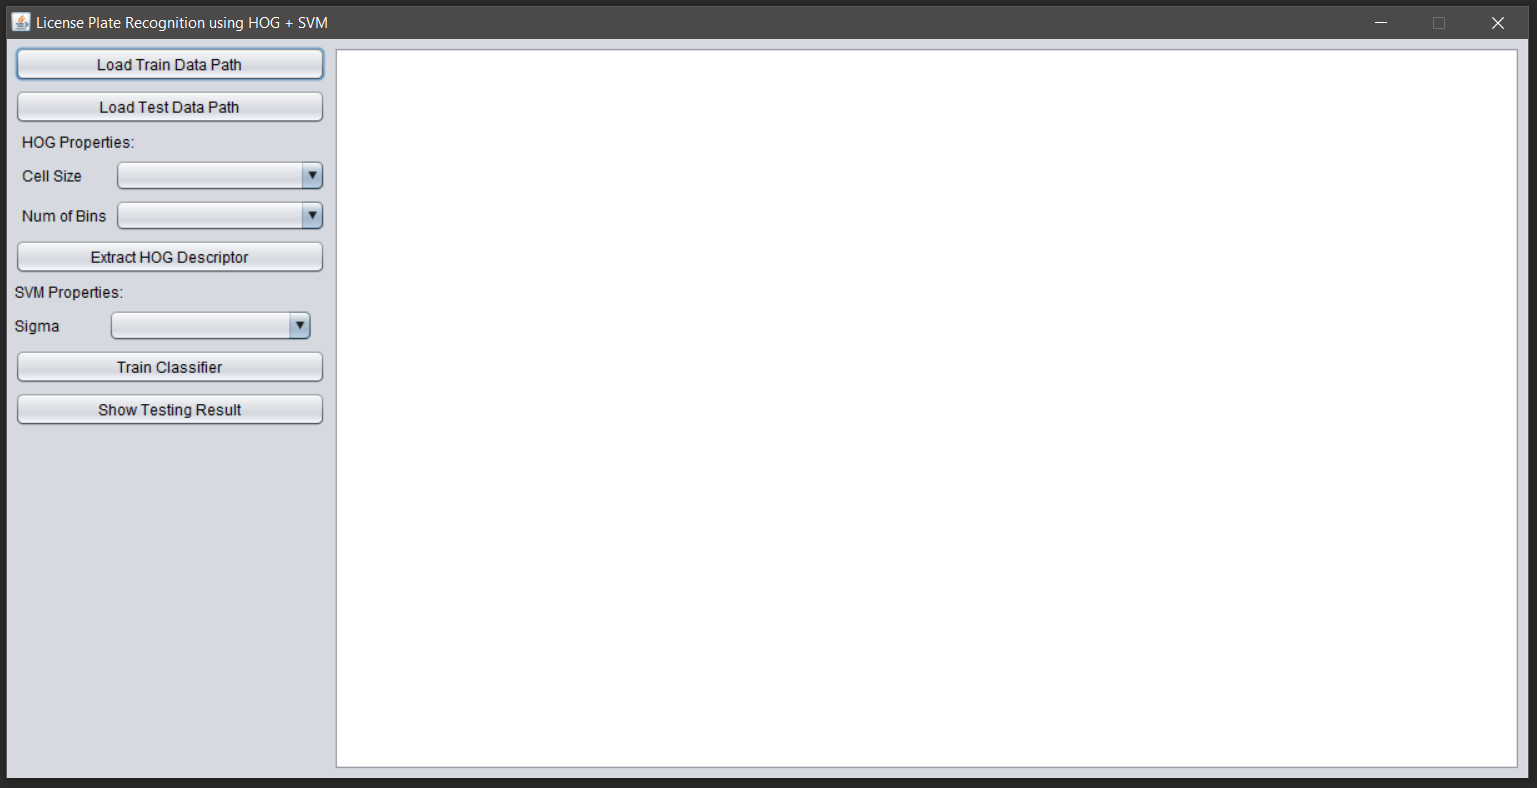
\includegraphics[width=14cm]{images/TampilanAntarmuka.png}
		\captionof{figure}{Tampilan antarmuka aplikasi pengenalan plat nomor kendaraan\\}
		\label{fig:TampilanAntarmuka}
	\end{minipage}
\end{adjustbox}\\
\\
\noindent Pada Gambar \ref{fig:TampilanAntarmuka}, terdapat beberapa tombol diantaranya adalah tombol \textit{Load Train Data Path}, \textit{Load Test Data Path}, \textit{Extract HOG Descriptor}, \textit{Train Classifier}, dan \textit{Show Testing Result}. Terdapat juga beberapa tombol \textit{dropdown} yang berfungsi untuk memilih nilai dari parameter metode HOG dan SVM. Untuk metode HOG tombol \textit{dropdown} yang tersedia adalah tombol \textit{dropdown} untuk memilih ukuran sel (\textit{Cell Size}) dan jumlah \textit{bins} yang akan digunakan (\textit{Num of Bins}). Sedangkan untuk metode SVM tombol \textit{dropdown} yang tersedia adalah tombol \textit{dropdown} untuk memilih nilai sigma yang akan digunakan. Tahapan proses pengenalan plat nomor kendaraan di aplikasi terbagi menjadi dua, yaitu proses \textit{training} dan proses \textit{testing}. Tahapan proses \textit{training} pada aplikasi adalah sebagai berikut:
\begin{enumerate}
\item Memasukkan \textit{path} dari kumpulan citra yang akan digunakan sebagai data latih untuk proses pengenalan karakter.
\item Memasukkan ukuran sel dan jumlah \textit{bin} yang digunakan untuk metode HOG dengan memilih menggunakan tombol \textit{dropdown Cell Size} dan tombol \textit{dropdown Num of Bins}.
\item Klik tombol \textit{Extract HOG Descriptor} untuk menjalankan proses ekstraksi fitur.
\item Klik tombol \textit{Train Classifier} untuk menjalankan proses \textit{training}.
\end{enumerate}
\begin{adjustbox}{width=1\textwidth}
	\noindent\begin{minipage}{\linewidth}
		\centering\framebox{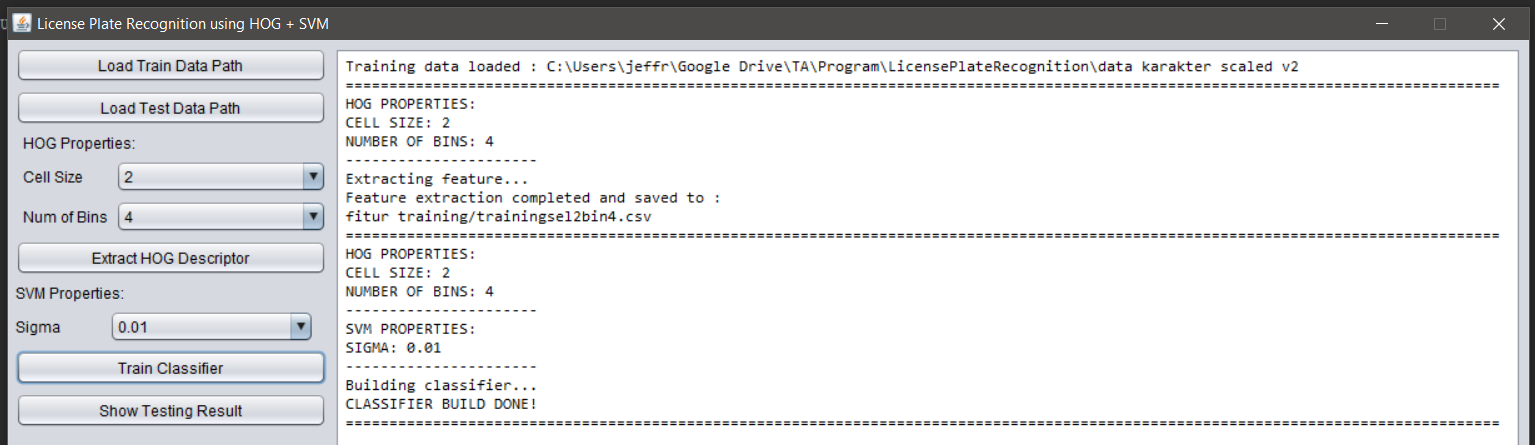
\includegraphics[width=14cm]{images/TampilanAntarmukaTraining.png}}
		\captionof{figure}{Tampilan antarmuka hasil \textit{training}\\}
		\label{fig:TampilanAntarmukaTraining}
	\end{minipage}
\end{adjustbox}\\
\\
\noindent Pada Gambar \ref{fig:TampilanAntarmukaTraining} aplikasi akan menampilkan \textit{path} dari folder citra yang akan digunakan sebagai data latih, ukuran sel dan jumlah \textit{bins} yang digunakan untuk metode HOG, pesan bahwa proses ekstraksi fitur sudah berjalan dan lokasi penyimpanan fitur, dan pesan bahwa proses \textit{training} sudah selesai.
\noindent Sedangkan untuk tahapan proses \textit{testing} pada aplikasi adalah sebagai berikut:
\begin{enumerate}
\item Lakukan proses \textit{training} terlebih dahulu.
\item Setelah proses \textit{training} selesai dilakukan, kemudian masukkan \textit{path} dari folder citra yang akan digunakan sebagai data uji.
\item Klik tombol \textit{Show Testing Result} untuk menjalankan proses testing otomatis.
\end{enumerate}
\begin{adjustbox}{width=1\textwidth}
	\noindent\begin{minipage}{\linewidth}
		\centering\framebox{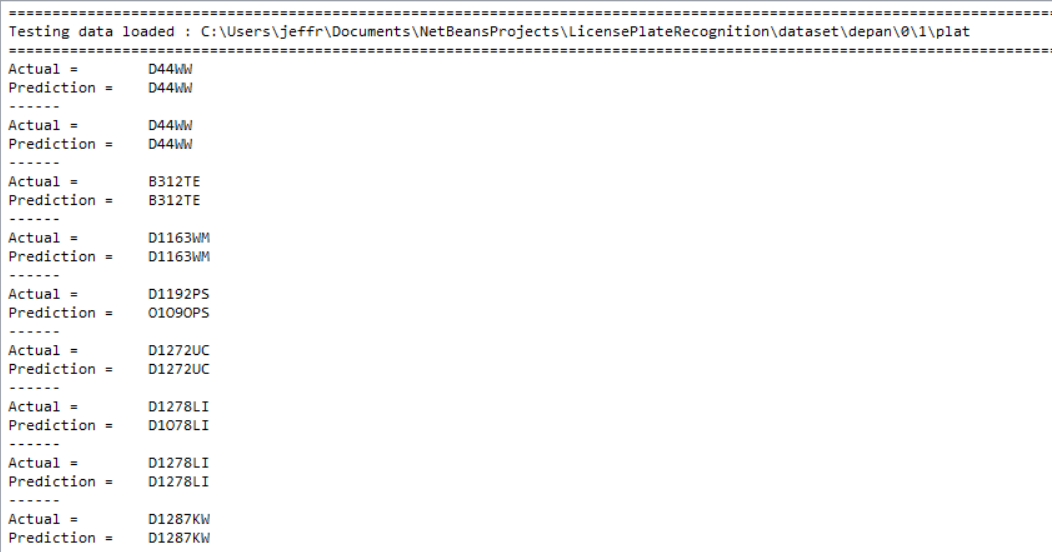
\includegraphics[width=14cm]{images/TampilanAntarmukaTesting1.png}}
		\captionof{figure}{Keluaran \textit{path} data untuk \textit{testing} dan hasil pengenalan plat}
		\label{fig:TampilanAntarmukaTesting1}
	\end{minipage}
\end{adjustbox}

\begin{adjustbox}{width=1\textwidth}
	\noindent\begin{minipage}{\linewidth}
		\centering\framebox{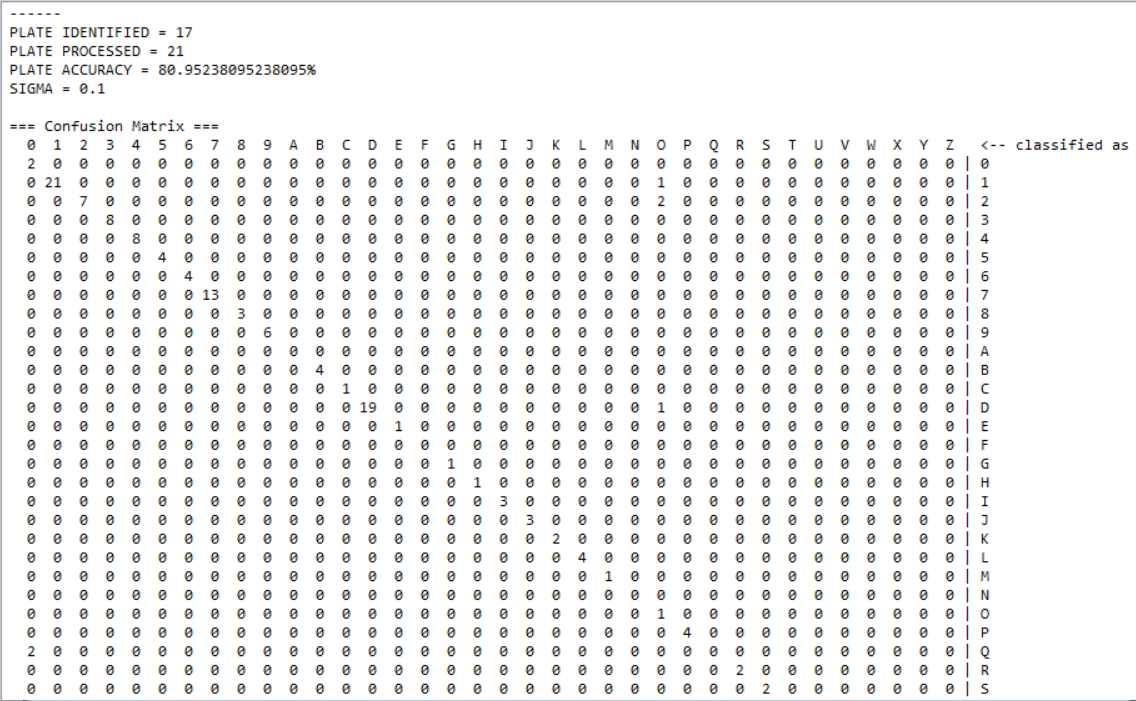
\includegraphics[width=14cm]{images/TampilanAntarmukaTesting2.png}}
		\captionof{figure}{Keluaran tingkat akurasi pengenalan plat dan \textit{Confusion Matrix}}
		\label{fig:TampilanAntarmukaTesting2}
	\end{minipage}
\end{adjustbox}

\begin{adjustbox}{width=1\textwidth}
	\noindent\begin{minipage}{\linewidth}
		\centering\framebox{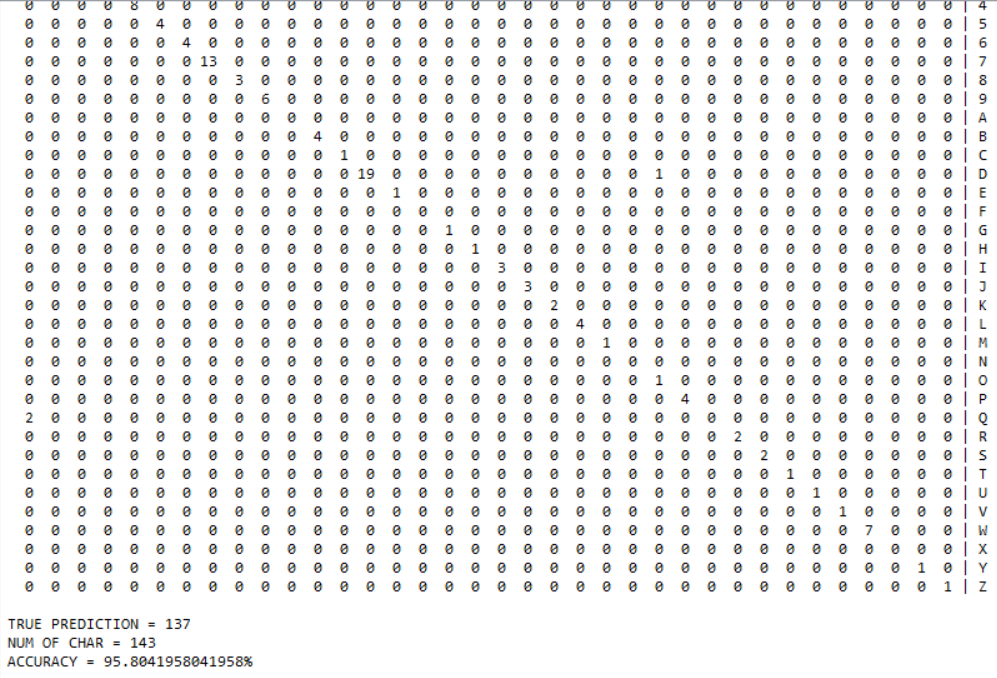
\includegraphics[width=14cm]{images/TampilanAntarmukaTesting3.png}}
		\captionof{figure}{Keluaran hasil tingkat akurasi pengenalan karakter\\}
		\label{fig:TampilanAntarmukaTesting3}
	\end{minipage}
\end{adjustbox}\\
\\
\noindent Pada Gambar \ref{fig:TampilanAntarmukaTesting1} aplikasi akan menampilkan \textit{path} dari folder citra yang akan digunakan sebagai data uji, teks asli dari plat nomor pada citra beserta hasil prediksi dari SVM, jumlah plat yang teridentifikasi dengan benar, jumlah total plat yang diproses, akurasi plat yang terdeteksi dan teridentifikasi dengan benar, hasil dari \textit{confusion matrix} untuk klasifikasi karakter, jumlah karakter yang terklasifikasi dengan benar, jumlah keseluruhan karakter, dan akurasi dari klasifikasi karakter.\\

\subsection{Implementasi Validasi Plat Kendaraan}
\noindent Bagian ini merupakan penjelasan implementasi tahap validasi plat kendaraan seperti yang disebutkan pada subbab 3.4.2.4, citra masukan berupa citra RGB mobil akan diproses untuk mendapatkan citra plat nomor dari citra RGB mobil. Berikut ini merupakan langkah pemrosesan citra dimulai dari masukan citra RGB mobil hingga menjadi citra plat.
\begin{enumerate}
	\item Baca citra RGB mobil dengan menggunakan \textit{Imgcodecs.imread()}. Parameter \textit{method} tersebut adalah lokasi citra yang akan diproses.
	\item Ubah citra RGB menjadi citra \textit{grayscale} dengan menggunakan \textit{Imgproc.cvtColor(mat1, mat2, Imgproc.COLORRGB2GRAY)}. Dengan parameter \textit{mat1} merupakan citra RGB dan \textit{mat2} adalah penampung citra hasil \textit{grayscale} dan \textit{COLORRBG2GRAY} adalah kode konversi \textit{color space} yang digunakan, kode yang digunakan adalah untuk mengkonversi citra RGB yang merupakan citra dengan 3 \textit{channel} warna menjadi citra dengan 1 \textit{channel} warna.
	\item Lakukan proses deteksi tepi \textit{Canny} dengan menggunakan \textit{Imgproc.Canny(gray, edge)}. Dengan parameter \textit{gray} adalah citra hasil \textit{grayscale} dan parameter \textit{edge} adalah penampung citra hasil deteksi tepi \textit{Canny}.
	\item Lakukan proses \textit{Hough Transform} sebanyak dua kali, yang pertama untuk mencari kandidat garis vertikal dengan \textit{range} $\theta$ -90 sampai dengan -85 derajat dan yang kedua adalah untuk mencari garis horizontal dengan \textit{range} $\theta$ -10 sampai dengan 10 derajat. Masing-masing dari kandidat garis vertikal dan horizontal disimpan dalam variabel dengan jenis \textit{ArrayList$<$Line$>$}.
	\item Untuk setiap elemen dalam \textit{ArrayList} yang berisi kandidat garis vertikal. Lakukan perbandingan antar elemen dengan membandingkan garis mana yang lebih kiri dan mana yang lebih kanan, kemudian dihitung lebar dari area yang dibatasi oleh kedua garis tersebut, apabila ukurannya berada dalam kisaran 255 - 390 piksel. Maka koordinat x dari titik awal kedua garis tersebut akan disimpan ke dalam matriks 2 dimensi yang berfungsi untuk menampung batas kiri, kanan, atas, dan bawah dari kandidat area plat.
	\item Untuk setiap elemen dalam \textit{ArrayList} yang berisi kandidat garis horizontal. Lakukan perbandingan antar elemen dengan membandingkan garis mana yang lebih atas dan mana yang lebih bawah, kemudian pasangkan dengan garis batas kiri dan kanan pada \textit{array} penampung kandidat batas kiri dan kanan plat nomor, kemudian hitung tinggi dari area yang dibatasi kedua garis horizontal, apabila berada di kisaran 85 - 130 piksel, maka koordinat y dari titik awal kedua garis tersebut akan ditambahkan pada elemen matriks yang berisi kandidat batas kiri dan kanan tadi, sehingga matriks 2 dimensi akan berisi koordinat titik yang merupakan area plat.
	\item Jika kandidat masih lebih dari satu kandidat, maka koordinat yang dipakai adalah koordinat yang rasio tinggi terhadap lebarnya paling mendekati 0.33.
	\item Kemudian lakukan pemotongan citra RGB dengan menggunakan koordinat yang didapat, dan hasil dari proses ini adalah citra plat.\\
\end{enumerate}

\section{Pengujian}
\noindent Pada bagian ini, akan dilakukan berbagai skenario pengujian dengan beragam parameter dari metode HOG. Tujuan dari penelitian ini adalah untuk menerapkan metode HOG pada proses ekstraksi fitur karakter pada sistem pengenalan karakter, oleh karena itu perlu diketahui berapa ukuran sel, ukuran blok, dan jumlah \textit{bin} yang akan menghasilkan fitur yang paling baik untuk akurasi pengenalan karakter. Pengujian ini akan dilakukan dengan data latih sebanyak 117 citra karakter hasil segmentasi dari plat nomor untuk 36 kelas karakter yang terdiri dari 10 kelas angka dan 26 kelas huruf, dimana setiap kelas karakter memiliki jumlah data latih sebanyak 3-5 citra.

\noindent Fitur dari metode \textit{HOG} akan digunakan pada proses klasifikasi karakter menggunakan \textit{library} SVM dari Weka dan akan diukur akurasinya menggunakan \textit{Confusion Matrix}. Adapun nilai dari setiap parameter yang akan digunakan untuk kombinasi, yaitu:
\begin{enumerate}
	\item Ukuran sel yang akan digunakan (dalam satuan piksel) : 2, 4, 8, 16
	\item Jumlah \textit{bin} yang akan digunakan : 4, 6, 9, 18
	\item Nilai \textit{sigma} pada metode \textit{SVM} yang akan digunakan: 0.01, 0.1, 1
	\item Campuran : Kombinasi parameter yang menghasilkan akurasi paling optimal untuk setiap karakter.\\
\end{enumerate}
%\noindent Adapun untuk nilai sigma pada metode \textit{SVM} yang digunakan dalam kombinasi adalah 0.01, 0.1, dan 1.

%\noindent Setelah setiap kombinasi ukuran sel, jumlah \textit{bin}, dan nilai sigma diuji, akan dipilih kombinasi parameter yang menghasilkan akurasi paling optimal untuk setiap karakter. Kemudian beberapa kombinasi parameter tersebut akan digabungkan dan diuji kembali, tujuannya untuk menilai apakah gabungan dari beberapa kombinasi parameter tersebut dapat meningkatkan akurasi.\\

\subsection{Pengujian Kombinasi Parameter}
\noindent Pada skenario pengujian ini, pengujian akan dilakukan dengan menggunakan ukuran sel berukuran 2 $\times$ 2 piksel, 4 $\times$ 4 piksel, 8 $\times$ 8 piksel, dan 16 $\times$ 16 piksel. Setiap ukuran sel akan menggunakan ukuran blok 2 $\times$ 2 sel. Jumlah bin yang akan digunakan adalah 4, 6, 9, dan 18. Sedangkan untuk nilai sigma pada metode \textit{SVM} yang akan digunakan adalah 0.01, 0.1, dan 1. Berikut adalah hasil pengujian untuk setiap kombinasi parameter tersebut:

%\begin{longtable}[c]{|c|c|c|c|c|}
%	\caption{Hasil Pengujian dengan ukuran sel 2 $\times$ 2 piksel}
%	\label{tab:HasilPengujianSel2}\\
%	\hline
%	\multicolumn{3}{|c|}{Parameter} &                                &                                \\ \cline{1-3}
%	CellSize   & NumBins   & Sigma  & \multirow{-2}{*}{CRR}          & \multirow{-2}{*}{OVR}          \\ \hline
%	\endhead
%	%
%	2          & 4         & 0.01   & {\color[HTML]{FE0000} 58.52\%} & {\color[HTML]{FE0000} 10.34\%} \\ \hline
%	2          & 4         & 0.1    & 26.13\%                        & 0\%                            \\ \hline
%	2          & 4         & 1      & 18.18\%                        & 0\%                            \\ \hline
%	2          & 6         & 0.01   & 50\%                           & 6.89\%                         \\ \hline
%	2          & 6         & 0.1    & 25.56\%                        & 0\%                            \\ \hline
%	2          & 6         & 1      & 18.18\%                        & 0\%                            \\ \hline
%	2          & 9         & 0.01   & 48.29\%                        & 3.44\%                         \\ \hline
%	2          & 9         & 0.1    & 25\%                           & 0\%                            \\ \hline
%	2          & 9         & 1      & 18.18\%                        & 0\%                            \\ \hline
%	2          & 18        & 0.01   & 44.88\%                        & 3.44\%                         \\ \hline
%	2          & 18        & 0.1    & 25\%                           & 0\%                            \\ \hline
%	2          & 18        & 1      & 18.18\%                        & 0\%                            \\ \hline
%\end{longtable}
%\begin{longtable}[c]{|r|r|r|r|r|}
%	\caption{Pengujian dengan ukuran sel 2 $\times$ 2 piksel}
%	\label{tab:HasilPengujianSel2}\\
%	\hline
%	\multicolumn{3}{|c|}{Parameter} &                                &                                \\ \cline{1-3}
%	CellSize   & NumBins   & Sigma  & \multicolumn{1}{c|}{\multirow{-2}{*}{CRR}} & \multicolumn{1}{c|}{\multirow{-2}{*}{OVR}} \\ \hline
%	\endhead
%	%
%	2          & 4         & 0.01   & {\color[HTML]{FE0000} 61.53\%} & {\color[HTML]{FE0000} 14.28\%} \\ \hline
%	2          & 4         & 0.1    & 28.67\%                        & 0\%                            \\ \hline
%	2          & 4         & 1      & 20.27\%                        & 0\%                            \\ \hline
%	2          & 6         & 0.01   & 53.84\%                        & 9.52\%                         \\ \hline
%	2          & 6         & 0.1    & 27.97\%                        & 0\%                            \\ \hline
%	2          & 6         & 1      & 20.27\%                        & 0\%                            \\ \hline
%	2          & 9         & 0.01   & 52.44\%                        & 4.76\%                         \\ \hline
%	2          & 9         & 0.1    & 27.27\%                        & 0\%                            \\ \hline
%	2          & 9         & 1      & 20.27\%                        & 0\%                            \\ \hline
%	2          & 18        & 0.01   & 48.25\%                        & 4.76\%                         \\ \hline
%	2          & 18        & 0.1    & 27.97\%                        & 0\%                            \\ \hline
%	2          & 18        & 1      & 20.27\%                        & 0\%                            \\ \hline
%\end{longtable}
\begin{adjustbox}{width=1\textwidth}
	\noindent\begin{minipage}{\linewidth}
		\centering\framebox{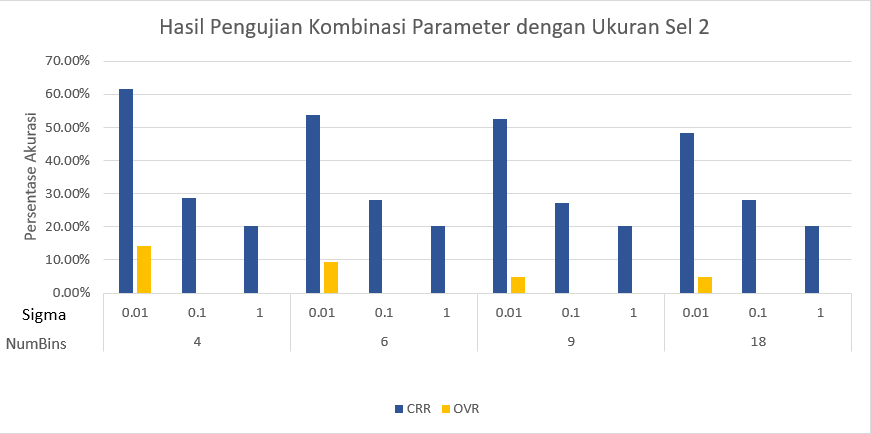
\includegraphics[width=14cm]{images/HasilPengujianUkuranSel2.png}}
		\captionof{figure}{Hasil Pengujian Kombinasi Parameter dengan Ukuran Sel 2\\}
		\label{fig:HasilPengujianUkuranSel2}
	\end{minipage}
\end{adjustbox}

\noindent Berdasarkan Gambar \ref{fig:HasilPengujianUkuranSel2}, dapat disimpulkan bahwa tingkat akurasi pengenalan karakter (CRR) maksimal yang didapatkan apabila menggunakan ukuran sel 2 $\times$ 2 piksel adalah 61.53\%. Kombinasi parameter yang digunakan untuk mencapai hasil tersebut adalah ukuran sel 2 $\times$ 2 piksel, jumlah \textit{bin} sebanyak 4 sehingga besar setiap \textit{bin} adalah 45 derajat, kemudian nilai \textit{sigma} yang digunakan untuk metode \textit{SVM} adalah 0.01. Dengan citra karakter masukan berukuran 32 $\times$ 32 piksel. Maka panjang vektor fitur dari \textit{HOG descriptor} yang dihasilkan adalah 3600 fitur.

\noindent Grafik batang berwarna biru menunjukkan tingkat akurasi pengenalan karakter (CRR). CRR sendiri merupakan akronim dari \textit{Character Recognition Rate} yang memiliki rumus jumlah karakter yang dikenali dibagi dengan keseluruhan karakter yang terdeteksi. Berdasarkan hasil CRR tertinggi pada Gambar \ref{fig:HasilPengujianUkuranSel2}, dari 143 karakter yang terdeteksi, sebanyak 88 di antaranya dapat diklasifikasikan dengan baik. Grafik batang berwarna kuning menunjukkan performa keseluruhan aplikasi (OVR). OVR merupakan akronim dari \textit{Overall Performance} yang memiliki rumus jumlah plat nomor yang terdeteksi dan dikenali dengan benar dibagi dengan keseluruhan jumlah plat nomor yang ada. Berdasarkan hasil OVR tertinggi dari Gambar \ref{fig:HasilPengujianUkuranSel2}, dari 21 plat nomor yang terdeteksi, hanya 3 plat nomor yang dapat dikenali dengan baik. 

\noindent Tabel \ref{tab:hasilklasifikasisel2} merupakan tabel yang menunjukkan hasil klasifikasi karakter dengan parameter HOG (\textit{CellSize} dan \textit{NumBins}) masing-masing 2 dan 4, dan nilai \textit{sigma} untuk metode \textit{SVM} 0.01.

\begin{longtable}[c]{|r|r|r|r|r|}
	\caption{Klasifikasi karakter dengan parameter CellSize = 2, NumBins = 4, dan Sigma = 0.01}
	\label{tab:hasilklasifikasisel2}\\
	\hline
	\textbf{No} & \textbf{Karakter} & \textbf{Prediksi Benar} & \textbf{Prediksi Salah} & \textbf{Akurasi} \\ \hline
	\endfirsthead
	\hline
	\textbf{No} & \textbf{Karakter} & \textbf{Prediksi Benar} & \textbf{Prediksi Salah} & \textbf{Akurasi} \\ \hline
	\endhead
	1           & 0                 & 2                       & 0                       &100.00\%            \\ \hline
	2           & 1                 & 15                       & 7                       &68.18\%            \\ \hline
	3           & 2                 & 6                       & 3                       &66.67\%            \\ \hline
	4           & 3                 & 2                       & 6                       &25.00\%            \\ \hline
	5           & 4                 & 3                       & 5                       &37.50\%            \\ \hline
	6           & 5                 & 2                       & 2                       &50.00\%            \\ \hline
	7           & 6                 & 1                       & 3                       &25.00\%            \\ \hline
	8           & 7                 & 6                       & 7                       &46.15\%            \\ \hline
	9           & 8                 & 1                       & 2                       &33.33\%            \\ \hline
	10           & 9                 & 2                       & 4                       &33.33\%            \\ \hline
	11           & A                 & 0                       & 0                       & -            \\ \hline
	12           & B                 & 1                       & 3                       &25.00\%            \\ \hline
	13           & C                 & 1                       & 0                       &100.00\%            \\ \hline
	14           & D                 & 20                       & 0                       &100.00\%            \\ \hline
	15           & E                 & 1                       & 0                       &100.00\%            \\ \hline
	16           & F                 & 0                       & 0                       & -            \\ \hline
	17           & G                 & 1                       & 0                       &100.00\%            \\ \hline
	18           & H                 & 1                       & 0                       &100.00\%            \\ \hline
	19           & I                 & 1                       & 2                       &33.33\%            \\ \hline
	20           & J                 & 2                       & 1                       &66.67\%            \\ \hline
	21           & K                 & 2                       & 0                       &100.00\%            \\ \hline
	22           & L                 & 4                       & 0                       &100.00\%            \\ \hline
	23           & M                 & 1                       & 0                       &100.00\%            \\ \hline
	24           & N                 & 0                       & 0                       & -            \\ \hline
	25           & O                 & 1                       & 0                       &100.00\%            \\ \hline
	26           & P                 & 1                       & 3                       &25.00\%            \\ \hline
	27           & Q                 & 2                       & 0                       &100.00\%            \\ \hline
	28           & R                 & 1                       & 1                       &50.00\%            \\ \hline
	29           & S                 & 1                       & 1                       &50.00\%            \\ \hline
	30           & T                 & 1                       & 0                       &100.00\%            \\ \hline
	31           & U                 & 1                       & 0                       &100.00\%            \\ \hline
	32           & V                 & 1                       & 0                       &100.00\%            \\ \hline
	33           & W                 & 2                       & 5                       &28.57\%            \\ \hline
	34           & X                 & 0                       & 0                       & -            \\ \hline
	35           & Y                 & 1                       & 0                       &100.00\%            \\ \hline
	36           & Z                 & 1                       & 0                       &100.00\%            \\ \hline
\end{longtable}

\noindent Dengan tingkat akurasi pengenalan karakter (\textit{Character Recognition Rate}) sebesar 61.53\%, dapat dilihat pada tabel \ref{tab:hasilklasifikasisel2} bahwa dari 36  karakter yang ada, yang dapat diprediksi dengan benar 100\% adalah sebanyak 16 karakter, terdapat juga beberapa karakter yang memiliki akurasi pengenalan yang rendah, diantaranya adalah angka 3, angka 4, angka 6, angka 7, angka 8, angka 9, huruf B, huruf I, huruf P, dan huruf W. Dari hasil akurasi klasifikasi di atas, dapat disimpulkan bahwa penggunaan ukuran sel 2 $\times$ 2 piksel kurang tepat untuk digunakan dalam proses ekstraksi fitur HOG dalam sistem pengenalan karakter ini.

%\subsection{Pengujian dengan Ukuran Sel 4}
%\noindent Pada bagian ini, pengujian akan dilakukan dengan menggunakan ukuran sel berukuran 4 $\times$ 4 piksel dan ukuran blok 2 $\times$ 2 sel (8 $\times$ 8 piksel). Jumlah bin yang akan digunakan adalah 4, 6, 9, dan 18. Sedangkan untuk nilai sigma pada metode \textit{SVM} yang akan digunakan adalah 0.01, 0.1, dan 1. Berikut adalah hasil pengujian untuk setiap kombinasi parameter tersebut:
%\begin{longtable}[c]{|c|c|c|}
%	\caption{Hasil Pengujian dengan ukuran sel 4 $\times$ 4 piksel}
%	\label{tab:HasilPengujianSel4}\\
%	\hline
%	\begin{tabular}[c]{@{}c@{}}Parameter\\ (CellSize, NumBins, Sigma)\end{tabular} & CRR     & OVR     \\ \hline
%	\endhead
%	%
%	(4, 4, 0.01)                                                                   & 86.36\% & 27.58\% \\ \hline
%	(4, 4, 0.1)                                                                    & 47.72\% & 0\%     \\ \hline
%	(4, 4, 1)                                                                      & 26.13\% & 0\%     \\ \hline
%	(4, 6, 0.01)                                                                   & 85.22\% & 31.03\%  \\ \hline
%	(4, 6, 0.1)                                                                    & 40.90\% & 0\%     \\ \hline
%	(4, 6, 1)                                                                      & 25\%    & 0\%     \\ \hline
%	(4, 9, 0.01)                                                                   & {\color[HTML]{FE0000} 89.77\%} & {\color[HTML]{FE0000} 37.93\%}  \\ \hline
%	(4, 9, 0.1)                                                                    & 40.90\% & 0\%     \\ \hline
%	(4, 9, 1)                                                                      & 23.86\% & 0\%     \\ \hline
%	(4, 18, 0.01)                                                                  & 84.09\% & 34.48\%  \\ \hline
%	(4, 18, 0.1)                                                                   & 40.90\% & 0\%     \\ \hline
%	(4, 18, 1)                                                                     & 24.43\% & 0\%     \\ \hline
%\end{longtable}
%\begin{longtable}[c]{|r|r|r|r|r|}
%	\caption{Pengujian dengan ukuran sel 4 $\times$ 4 piksel}
%	\label{tab:HasilPengujianSel4}\\
%	\hline
%	\multicolumn{3}{|c|}{Parameter} &                                &                                \\ \cline{1-3}
%	CellSize   & NumBins   & Sigma  & \multicolumn{1}{c|}{\multirow{-2}{*}{CRR}} & \multicolumn{1}{c|}{\multirow{-2}{*}{OVR}} \\ \hline
%	\endhead
%	%
%	4          & 4         & 0.01   & 88.11\%                        & 38.09\% \\ \hline
%	4          & 4         & 0.1    & 50.34\%                        & 0\%                            \\ \hline
%	4          & 4         & 1      & 27.97\%                        & 0\%                            \\ \hline
%	4          & 6         & 0.01   & 86.71\%                        & 42.85\%                         \\ \hline
%	4          & 6         & 0.1    & 44.05\%                        & 0\%                            \\ \hline
%	4          & 6         & 1      & 26.57\%                        & 0\%                            \\ \hline
%	4          & 9         & 0.01   & {\color[HTML]{FE0000} 90.20\%} & {\color[HTML]{FE0000} 52.38\%} \\ \hline
%	4          & 9         & 0.1    & 44.05\%                        & 0\%                            \\ \hline
%	4          & 9         & 1      & 25.87\%                        & 0\%                            \\ \hline
%	4          & 18        & 0.01   & 87.41\%                        & 47.61\%                         \\ \hline
%	4          & 18        & 0.1    & 44.05\%                        & 0\%                            \\ \hline
%	4          & 18        & 1      & 25.87\%                        & 0\%                            \\ \hline
%\end{longtable}
\begin{adjustbox}{width=1\textwidth}
	\noindent\begin{minipage}{\linewidth}
		\centering\framebox{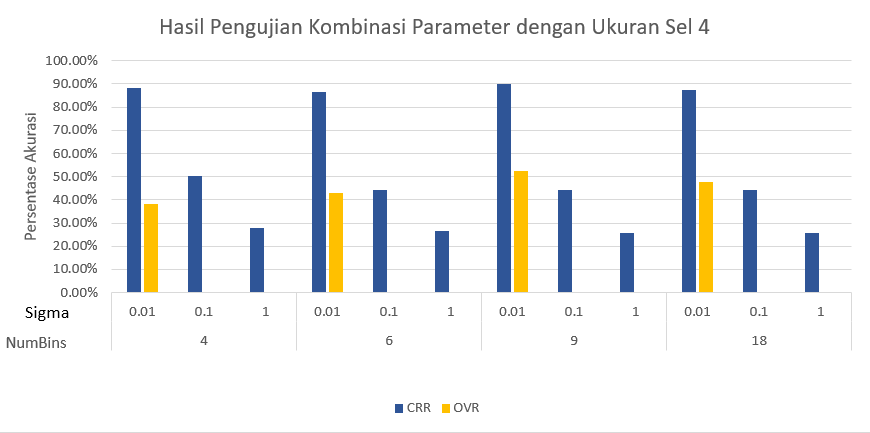
\includegraphics[width=14cm]{images/HasilPengujianUkuranSel4.png}}
		\captionof{figure}{Hasil Pengujian Kombinasi Parameter dengan Ukuran Sel 4\\}
		\label{fig:HasilPengujianUkuranSel4}
	\end{minipage}
\end{adjustbox}

\noindent Berdasarkan Gambar \ref{fig:HasilPengujianUkuranSel4}, dapat disimpulkan bahwa tingkat akurasi pengenalan karakter (CRR) maksimal yang didapatkan apabila menggunakan ukuran sel 4 $\times$ 4 piksel adalah 90.20\%. Kombinasi parameter yang digunakan untuk mencapai hasil tersebut adalah ukuran sel 4 $\times$ 4 piksel, jumlah \textit{bin} sebanyak 9 sehingga besar setiap \textit{bin} adalah 20 derajat, kemudian nilai \textit{sigma} yang digunakan untuk metode \textit{SVM} adalah 0.01. Dengan citra karakter masukan berukuran 32 $\times$ 32 piksel. Maka panjang vektor fitur dari \textit{HOG descriptor} yang dihasilkan adalah 1764 fitur. Jika dibandingkan dengan pengujian sebelumnya, jumlah fitur yang lebih sedikit justru mampu mendapatkan akurasi pengenalan karakter yang lebih baik.

\noindent Berdasarkan hasil CRR tertinggi pada Gambar \ref{fig:HasilPengujianUkuranSel4}, dari 143 karakter yang terdeteksi, sebanyak 129 di antaranya dapat diklasifikasikan dengan baik. Sedangkan dari hasil OVR tertinggi pada Gambar \ref{fig:HasilPengujianUkuranSel4}, dari 21 plat nomor yang terdeteksi, 11 plat nomor dapat dikenali dengan baik, hal ini merupakan peningkatan apabila dibandingkan dengan hasil pengujian sebelumnya, namun masih cukup banyak plat yang tidak dapat dikenali dengan baik. 

\noindent Tabel \ref{tab:hasilklasifikasisel4} merupakan tabel yang menunjukkan hasil klasifikasi karakter dengan parameter HOG (\textit{CellSize} dan \textit{NumBins}) masing-masing 4 dan 9, dan nilai \textit{sigma} untuk metode \textit{SVM} 0.01.

\begin{longtable}[c]{|r|r|r|r|r|}
	\caption{Klasifikasi karakter dengan parameter CellSize = 4, NumBins = 9, dan Sigma = 0.01}
	\label{tab:hasilklasifikasisel4}\\
	\hline
	\textbf{No} & \textbf{Karakter} & \textbf{Prediksi Benar} & \textbf{Prediksi Salah} & \textbf{Akurasi} \\ \hline
	\endhead
	1           & 0                 & 0                       & 2                       &0.00\%            \\ \hline
	2           & 1                 & 18                       & 4                       &81.82\%            \\ \hline
	3           & 2                 & 7                       & 2                       &77.78\%            \\ \hline
	4           & 3                 & 8                       & 0                       &100.00\%            \\ \hline
	5           & 4                 & 8                       & 0                       &100.00\%            \\ \hline
	6           & 5                 & 4                       & 0                       &100.00\%            \\ \hline
	7           & 6                 & 4                       & 0                       &100.00\%            \\ \hline
	8           & 7                 & 13                       & 0                       &100.00\%            \\ \hline
	9           & 8                 & 3                       & 0                       &100.00\%            \\ \hline
	10           & 9                 & 6                       & 0                       &100.00\%            \\ \hline
	11           & A                 & 0                       & 0                       & -            \\ \hline
	12           & B                 & 4                       & 0                       &100.00\%            \\ \hline
	13           & C                 & 1                       & 0                       &100.00\%            \\ \hline
	14           & D                 & 19                       & 1                       &95.00\%            \\ \hline
	15           & E                 & 1                       & 0                       &100.00\%            \\ \hline
	16           & F                 & 0                       & 0                       & -            \\ \hline
	17           & G                 & 1                       & 0                       &100.00\%            \\ \hline
	18           & H                 & 1                       & 0                       &100.00\%            \\ \hline
	19           & I                 & 3                       & 0                       &100.00\%            \\ \hline
	20           & J                 & 2                       & 1                       &66.67\%            \\ \hline
	21           & K                 & 2                       & 0                       &100.00\%            \\ \hline
	22           & L                 & 4                       & 0                       &100.00\%            \\ \hline
	23           & M                 & 1                       & 0                       &100.00\%            \\ \hline
	24           & N                 & 0                       & 0                       & -            \\ \hline
	25           & O                 & 1                       & 0                       &100.00\%            \\ \hline
	26           & P                 & 4                       & 0                       &100.00\%            \\ \hline
	27           & Q                 & 0                       & 2                       &0.00\%            \\ \hline
	28           & R                 & 2                       & 0                       &100.00\%            \\ \hline
	29           & S                 & 2                       & 0                       &100.00\%            \\ \hline
	30           & T                 & 1                       & 0                       &100.00\%            \\ \hline
	31           & U                 & 0                       & 1                       &0.00\%            \\ \hline
	32           & V                 & 1                       & 0                       &100.00\%            \\ \hline
	33           & W                 & 6                       & 1                       &85.71\%            \\ \hline
	34           & X                 & 0                       & 0                       & -            \\ \hline
	35           & Y                 & 1                       & 0                       &100.00\%            \\ \hline
	36           & Z                 & 1                       & 0                       &100.00\%            \\ \hline
\end{longtable}

\noindent Dengan tingkat akurasi pengenalan karakter (\textit{Character Recognition Rate}) sebesar 90.20\%, dapat dilihat pada tabel \ref{tab:hasilklasifikasisel4} bahwa dari 36  karakter yang ada, yang dapat diprediksi dengan benar 100\% adalah sebanyak 24 karakter, terdapat juga beberapa karakter yang memiliki akurasi pengenalan yang rendah, diantaranya adalah angka 0, huruf Q, dan huruf U. Dari hasil akurasi klasifikasi di atas, dapat  disimpulkan bahwa penggunaan ukuran sel 4 $\times$ 4 piksel sudah dapat meningkatkan akurasi pengenalan karakter namun masih belum optimal.

%\subsection{Pengujian dengan Ukuran Sel 8}
%\noindent Pada bagian ini, pengujian akan dilakukan dengan menggunakan ukuran sel berukuran 8 $\times$ 8 piksel dan ukuran blok 2 $\times$ 2 sel (16 $\times$ 16 piksel). Jumlah bin yang akan digunakan adalah 4, 6, 9, dan 18. Sedangkan untuk nilai sigma pada metode \textit{SVM} yang akan digunakan adalah 0.01, 0.1, dan 1. Berikut adalah hasil pengujian untuk setiap kombinasi parameter tersebut:
%\begin{longtable}[c]{|c|c|c|}
%	\caption{Hasil Pengujian dengan ukuran sel 8 $\times$ 8 piksel}
%	\label{tab:HasilPengujianSel8}\\
%	\hline
%	\begin{tabular}[c]{@{}c@{}}Parameter\\ (CellSize, NumBins, Sigma)\end{tabular} & CRR     & OVR     \\ \hline
%	\endhead
%	%
%	(8, 4, 0.01)                                                                   & 15.90\% & 0\% \\ \hline
%	(8, 4, 0.1)                                                                    & 93.18\% & 51.72\%     \\ \hline
%	(8, 4, 1)                                                                      & 46.02\% & 0\%     \\ \hline
%	(8, 6, 0.01)                                                                   & 21.02\% & 0\%  \\ \hline
%	(8, 6, 0.1)                                                                    & 93.18\% & 51.72\%     \\ \hline
%	(8, 6, 1)                                                                      & 42.61\% & 0\%     \\ \hline
%	(8, 9, 0.01)                                                                   & 28.40\% & 0\%  \\ \hline
%	(8, 9, 0.1)                                                                    & 93.75\% & 51.72\%     \\ \hline
%	(8, 9, 1)                                                                      & 39.20\% & 0\%     \\ \hline
%	(8, 18, 0.01)                                                                  & 21.59\% & 0\%  \\ \hline
%	(8, 18, 0.1)                                                                   & {\color[HTML]{FE0000} 94.88\%} & {\color[HTML]{FE0000} 58.62\%}     \\ \hline
%	(8, 18, 1)                                                                     & 40.34\% & 0\%     \\ \hline
%\end{longtable}
%\begin{longtable}[c]{|r|r|r|r|r|}
%	\caption{Pengujian dengan ukuran sel 8 $\times$ 8 piksel}
%	\label{tab:HasilPengujianSel8}\\
%	\hline
%	\multicolumn{3}{|c|}{Parameter} &                                &                                \\ \cline{1-3}
%	CellSize   & NumBins   & Sigma  & \multicolumn{1}{c|}{\multirow{-2}{*}{CRR}} & \multicolumn{1}{c|}{\multirow{-2}{*}{OVR}} \\ \hline
%	\endhead
%	%
%	8          & 4         & 0.01   & 17.48\%                        & 0\% \\ \hline
%	8          & 4         & 0.1    & 94.40\%                        & 71.42\%                            \\ \hline
%	8          & 4         & 1      & 48.95\%                        & 0\%                            \\ \hline
%	8          & 6         & 0.01   & 23.07\%                        & 0\%                         \\ \hline
%	8          & 6         & 0.1    & 94.40\%                        & 71.42\%                            \\ \hline
%	8          & 6         & 1      & 46.15\%                        & 0\%                            \\ \hline
%	8          & 9         & 0.01   & 29.37\%                        & 0\% \\ \hline
%	8          & 9         & 0.1    & 94.40\%                        & 71.42\%                            \\ \hline
%	8          & 9         & 1      & 41.95\%                        & 0\%                            \\ \hline
%	8          & 18        & 0.01   & 23.77\%                        & 0\%                         \\ \hline
%	8          & 18        & 0.1    & {\color[HTML]{FE0000} 95.80\%} & {\color[HTML]{FE0000} 80.95\%}                            \\ \hline
%	8          & 18        & 1      & 43.35\%                        & 0\%                            \\ \hline
%\end{longtable}
\begin{adjustbox}{width=1\textwidth}
	\noindent\begin{minipage}{\linewidth}
		\centering\framebox{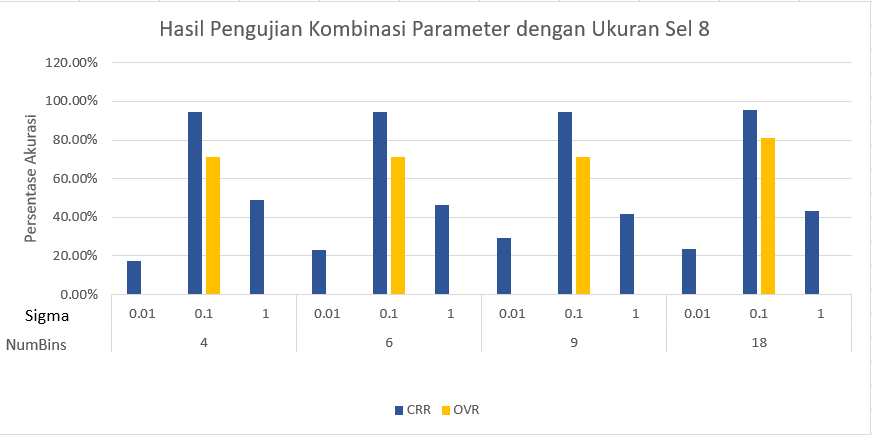
\includegraphics[width=14cm]{images/HasilPengujianUkuranSel8.png}}
		\captionof{figure}{Hasil Pengujian Kombinasi Parameter dengan Ukuran Sel 8\\}
		\label{fig:HasilPengujianUkuranSel8}
	\end{minipage}
\end{adjustbox}

\noindent Berdasarkan Gambar \ref{fig:HasilPengujianUkuranSel8}, dapat disimpulkan bahwa tingkat akurasi pengenalan karakter maksimal yang didapatkan apabila menggunakan ukuran sel 8 $\times$ 8 piksel adalah 95.80\%. Kombinasi parameter yang digunakan untuk mencapai hasil tersebut adalah ukuran sel 8 $\times$ 8 piksel, jumlah \textit{bin} sebanyak 18 sehingga besar setiap \textit{bin} adalah 10 derajat, kemudian nilai \textit{sigma} yang digunakan untuk metode \textit{SVM} adalah 0.1. Dengan citra karakter masukan berukuran 32 $\times$ 32 piksel. Maka panjang vektor fitur dari \textit{HOG descriptor} yang dihasilkan adalah 648 fitur. Sama seperti pengujian sebelumnya, jika dibandingkan dengan pengujian sebelumnya, jumlah fitur yang lebih sedikit justru mampu mendapatkan akurasi pengenalan karakter yang lebih baik.

\noindent Dari hasil CRR tertinggi pada Gambar \ref{fig:HasilPengujianUkuranSel8}, dari 143 karakter yang terdeteksi, sebanyak 137 di antaranya dapat diklasifikasikan dengan baik. Sedangkan dari hasil OVR tertinggi pada Gambar \ref{fig:HasilPengujianUkuranSel8} menunjukkan, dari 21 plat nomor yang terdeteksi, 17 plat nomor dapat dikenali dengan baik, hal ini merupakan peningkatan apabila dibandingkan dengan hasil pengujian sebelumnya.

\noindent Tabel \ref{tab:hasilklasifikasisel8} merupakan tabel yang menunjukkan hasil klasifikasi karakter dengan parameter HOG (\textit{CellSize} dan \textit{NumBins}) masing-masing 8 dan 18, dan nilai \textit{sigma} untuk metode \textit{SVM} 0.1.

\begin{longtable}[c]{|r|r|r|r|r|}
	\caption{Klasifikasi karakter dengan parameter CellSize = 8, NumBins = 18, dan Sigma = 0.1}
	\label{tab:hasilklasifikasisel8}\\
	\hline
	\textbf{No} & \textbf{Karakter} & \textbf{Prediksi Benar} & \textbf{Prediksi Salah} & \textbf{Akurasi} \\ \hline
	\endhead
	1           & 0                 & 2                       & 0                       &100.00\%            \\ \hline
	2           & 1                 & 21                       & 1                       &95.45\%            \\ \hline
	3           & 2                 & 7                       & 2                       &77.78\%            \\ \hline
	4           & 3                 & 8                       & 0                       &100.00\%            \\ \hline
	5           & 4                 & 8                       & 0                       &100.00\%            \\ \hline
	6           & 5                 & 4                       & 0                       &100.00\%            \\ \hline
	7           & 6                 & 4                       & 0                       &100.00\%            \\ \hline
	8           & 7                 & 13                       & 0                       &100.00\%            \\ \hline
	9           & 8                 & 3                       & 0                       &100.00\%            \\ \hline
	10           & 9                 & 6                       & 0                       &100.00\%            \\ \hline
	11           & A                 & 0                       & 0                       & -            \\ \hline
	12           & B                 & 4                       & 0                       &100.00\%            \\ \hline
	13           & C                 & 1                       & 0                       &100.00\%            \\ \hline
	14           & D                 & 19                       & 1                       &95.00\%            \\ \hline
	15           & E                 & 1                       & 0                       &100.00\%            \\ \hline
	16           & F                 & 0                       & 0                       & -            \\ \hline
	17           & G                 & 1                       & 0                       &100.00\%            \\ \hline
	18           & H                 & 1                       & 0                       &100.00\%            \\ \hline
	19           & I                 & 3                       & 0                       &100.00\%            \\ \hline
	20           & J                 & 3                       & 0                       &100.00\%            \\ \hline
	21           & K                 & 2                       & 0                       &100.00\%            \\ \hline
	22           & L                 & 4                       & 0                       &100.00\%            \\ \hline
	23           & M                 & 1                       & 0                       &100.00\%            \\ \hline
	24           & N                 & 0                       & 0                       & -            \\ \hline
	25           & O                 & 1                       & 0                       &100.00\%            \\ \hline
	26           & P                 & 4                       & 0                       &100.00\%            \\ \hline
	27           & Q                 & 0                       & 2                       &0.00\%            \\ \hline
	28           & R                 & 2                       & 0                       &100.00\%            \\ \hline
	29           & S                 & 2                       & 0                       &100.00\%            \\ \hline
	30           & T                 & 1                       & 0                       &100.00\%            \\ \hline
	31           & U                 & 1                       & 0                       &100.00\%            \\ \hline
	32           & V                 & 1                       & 0                       &100.00\%            \\ \hline
	33           & W                 & 7                       & 0                       &100.00\%            \\ \hline
	34           & X                 & 0                       & 0                       & -            \\ \hline
	35           & Y                 & 1                       & 0                       &100.00\%            \\ \hline
	36           & Z                 & 1                       & 0                       &100.00\%            \\ \hline
\end{longtable}

\noindent Dengan tingkat akurasi pengenalan karakter (\textit{Character Recognition Rate}) sebesar 95.80\%, dapat dilihat pada tabel \ref{tab:hasilklasifikasisel8} bahwa dari 36  karakter yang ada, yang dapat diprediksi dengan benar 100\% adalah sebanyak 29 karakter, dari karakter yang  tersisa, hanya satu karakter yang memiliki akurasi rendah, yaitu huruf Q yang mana dari 2 karakter yang terdapat di data \textit{testing}, tidak ada yang dapat diklasifikasikan dengan benar. Dari hasil pengujian ini dapat  disimpulkan bahwa penggunaan ukuran sel 8 $\times$ 8 piksel sudah dapat menghasilkan akurasi pengenalan karakter yang baik.\\

%\subsection{Pengujian dengan Ukuran Sel 16}
%\noindent Pada bagian ini, pengujian akan dilakukan dengan menggunakan ukuran sel berukuran 16 $\times$ 16 piksel dan ukuran blok 2 $\times$ 2 sel (32 $\times$ 32 piksel). Jumlah bin yang akan digunakan adalah 4, 6, 9, dan 18. Sedangkan untuk nilai sigma pada metode \textit{SVM} yang akan digunakan adalah 0.01, 0.1, dan 1. Berikut adalah hasil pengujian untuk setiap kombinasi parameter tersebut:
%\begin{longtable}[c]{|c|c|c|}
%	\caption{Hasil Pengujian dengan ukuran sel 16 $\times$ 16 piksel}
%	\label{tab:HasilPengujianSel16}\\
%	\hline
%	\begin{tabular}[c]{@{}c@{}}Parameter\\ (CellSize, NumBins, Sigma)\end{tabular} & CRR     & OVR     \\ \hline
%	\endhead
%	%
%	(16, 4, 0.01)                                                                   & 13.06\% & 0\% \\ \hline
%	(16, 4, 0.1)                                                                    & 18.75\% & 0\%     \\ \hline
%	(16, 4, 1)                                                                      & 84.09\% & 17.24\%     \\ \hline
%	(16, 6, 0.01)                                                                   & 13.06\% & 0\%  \\ \hline
%	(16, 6, 0.1)                                                                    & 22.72\% & 0\%     \\ \hline
%	(16, 6, 1)                                                                      & 84.09\% & 13.79\%     \\ \hline
%	(16, 9, 0.01)                                                                   & 13.06\% & 0\%  \\ \hline
%	(16, 9, 0.1)                                                                    & 28.97\% & 0\%     \\ \hline
%	(16, 9, 1)                                                                      & {\color[HTML]{FE0000} 86.36\%} & {\color[HTML]{FE0000} 27.58\%}     \\ \hline
%	(16, 18, 0.01)                                                                  & 13.06\% & 0\%  \\ \hline
%	(16, 18, 0.1)                                                                   & 23.29\% & 0\%     \\ \hline
%	(16, 18, 1)                                                                     & 85.79\% & 24.13\%     \\ \hline
%\end{longtable}
%\begin{longtable}[c]{|r|r|r|r|r|}
%	\caption{Pengujian dengan ukuran sel 16 $\times$ 16 piksel}
%	\label{tab:HasilPengujianSel16}\\
%	\hline
%	\multicolumn{3}{|c|}{Parameter} &                                &                                \\ \cline{1-3}
%	CellSize   & NumBins   & Sigma  & \multicolumn{1}{c|}{\multirow{-2}{*}{CRR}} & \multicolumn{1}{c|}{\multirow{-2}{*}{OVR}} \\ \hline
%	\endhead
%	%
%	16          & 4         & 0.01   & 13.98\%                        & 0\%                            \\ \hline
%	16          & 4         & 0.1    & 20.27\%                        & 0\%                            \\ \hline
%	16          & 4         & 1      & 83.91\%                        & 23.80\%                        \\ \hline
%	16          & 6         & 0.01   & 13.98\%                        & 0\%                            \\ \hline
%	16          & 6         & 0.1    & 25.17\%                        & 0\%                            \\ \hline
%	16          & 6         & 1      & 83.21\%                        & 19.04\%                        \\ \hline
%	16          & 9         & 0.01   & 13.98\%                        & 0\%                            \\ \hline
%	16          & 9         & 0.1    & 30.76\%                        & 0\%                            \\ \hline
%	16          & 9         & 1      & {\color[HTML]{FE0000} 86.71\%} & {\color[HTML]{FE0000} 38.09\%} \\ \hline
%	16          & 18        & 0.01   & 13.98\%                        & 0\%                            \\ \hline
%	16          & 18        & 0.1    & 25.87\%                        & 0\%                            \\ \hline
%	16          & 18        & 1      & 86.01\%                        & 33.33\%                        \\ \hline
%\end{longtable}
\begin{adjustbox}{width=1\textwidth}
	\noindent\begin{minipage}{\linewidth}
		\centering\framebox{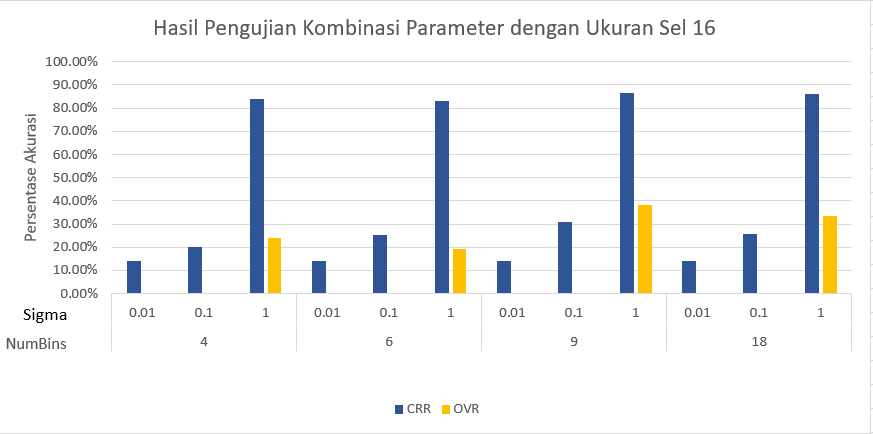
\includegraphics[width=14cm]{images/HasilPengujianUkuranSel16.png}}
		\captionof{figure}{Hasil Pengujian Kombinasi Parameter dengan Ukuran Sel 16\\}
		\label{fig:HasilPengujianUkuranSel16}
	\end{minipage}
\end{adjustbox}

\noindent Berdasarkan Gambar \ref{fig:HasilPengujianUkuranSel16}, dapat disimpulkan bahwa akurasi pengenalan karakter maksimal yang didapatkan apabila menggunakan ukuran sel 16 $\times$ 16 piksel adalah 86.71\%. Kombinasi parameter yang digunakan untuk mencapai hasil tersebut adalah ukuran sel 16 $\times$ 16 piksel, jumlah \textit{bin} sebanyak 9 sehingga besar setiap \textit{bin} adalah 20 derajat, kemudian nilai \textit{sigma} yang digunakan untuk metode \textit{SVM} adalah 1. Dengan citra karakter masukan berukuran 32 $\times$ 32 piksel. Maka panjang vektor fitur dari \textit{HOG descriptor} yang dihasilkan adalah 9 fitur. Berbeda dengan pengujian sebelumnya, kali ini jumlah fitur yang terlalu sedikit justru akan mengurangi akurasi dari proses pengenalan karakter yang sebelumnya sudah mencapai 95.80\%. 
%dari keseluruhan pengujian yang sudah dilakukan terhadap jumlah sel, dapat disimpulkan bahwa ukuran sel yang terlampau besar ataupun terlampau kecil pada penggunaan metode \textit{HOG} dapat mengurangi kualitas fitur yang dihasilkan sehingga akan berefek terhadap hasil klasifikasi.

\noindent Berdasarkan hasil CRR tertinggi pada Gambar \ref{fig:HasilPengujianUkuranSel16}, dari 143 karakter yang terdeteksi, sebanyak 123 di antaranya dapat diklasifikasikan dengan baik. Sedangkan berdasarkan hasil OVR tertinggi pada Gambar \ref{fig:HasilPengujianUkuranSel16} dari 21 plat nomor yang terdeteksi, 7 plat nomor dapat dikenali dengan baik, hal ini merupakan dampak dari penurunan akurasi pengenalan karakter.

\noindent Tabel \ref{tab:hasilklasifikasisel16} merupakan tabel yang menunjukkan hasil klasifikasi karakter dengan parameter HOG (\textit{CellSize} dan \textit{NumBins}) masing-masing 16 dan 9, dan nilai \textit{sigma} untuk metode \textit{SVM} 1.

\begin{longtable}[c]{|r|r|r|r|r|}
	\caption{Klasifikasi karakter dengan parameter CellSize = 16, NumBins = 9, dan Sigma = 1.0}
	\label{tab:hasilklasifikasisel16}\\
	\hline
	\textbf{No} & \textbf{Karakter} & \textbf{Prediksi Benar} & \textbf{Prediksi Salah} & \textbf{Akurasi} \\ \hline
	\endhead
	1           & 0                 & 2                       & 0                       &100.00\%            \\ \hline
	2           & 1                 & 20                       & 2                       &90.91\%            \\ \hline
	3           & 2                 & 6                       & 3                       &66.67\%            \\ \hline
	4           & 3                 & 8                       & 0                       &100.00\%            \\ \hline
	5           & 4                 & 8                       & 0                       &100.00\%            \\ \hline
	6           & 5                 & 4                       & 0                       &100.00\%            \\ \hline
	7           & 6                 & 4                       & 0                       &100.00\%            \\ \hline
	8           & 7                 & 13                       & 0                       &100.00\%            \\ \hline
	9           & 8                 & 3                       & 0                       &100.00\%            \\ \hline
	10           & 9                 & 6                       & 0                       &100.00\%            \\ \hline
	11           & A                 & 0                       & 0                       & -            \\ \hline
	12           & B                 & 3                       & 1                       &75.00\%            \\ \hline
	13           & C                 & 1                       & 0                       &100.00\%            \\ \hline
	14           & D                 & 19                       & 1                       &95.00\%            \\ \hline
	15           & E                 & 1                       & 0                       &100.00\%            \\ \hline
	16           & F                 & 0                       & 0                       & -            \\ \hline
	17           & G                 & 1                       & 0                       &100.00\%            \\ \hline
	18           & H                 & 1                       & 0                       &100.00\%            \\ \hline
	19           & I                 & 0                       & 3                       &0.00\%            \\ \hline
	20           & J                 & 3                       & 0                       &100.00\%            \\ \hline
	21           & K                 & 2                       & 0                       &100.00\%            \\ \hline
	22           & L                 & 4                       & 0                       &100.00\%            \\ \hline
	23           & M                 & 1                       & 0                       &100.00\%            \\ \hline
	24           & N                 & 0                       & 0                       & -            \\ \hline
	25           & O                 & 1                       & 0                       &100.00\%            \\ \hline
	26           & P                 & 4                       & 0                       &100.00\%            \\ \hline
	27           & Q                 & 0                       & 2                       &0.00\%            \\ \hline
	28           & R                 & 2                       & 0                       &100.00\%            \\ \hline
	29           & S                 & 2                       & 0                       &100.00\%            \\ \hline
	30           & T                 & 1                       & 0                       &100.00\%            \\ \hline
	31           & U                 & 1                       & 0                       &100.00\%            \\ \hline
	32           & V                 & 1                       & 0                       &100.00\%            \\ \hline
	33           & W                 & 0                       & 7                       &0.00\%            \\ \hline
	34           & X                 & 0                       & 0                       & -            \\ \hline
	35           & Y                 & 1                       & 0                       &100.00\%            \\ \hline
	36           & Z                 & 1                       & 0                       &100.00\%            \\ \hline
\end{longtable}

\noindent Dengan tingkat akurasi pengenalan karakter (\textit{Character Recognition Rate}) sebesar 86.71\%, dapat dilihat pada tabel \ref{tab:hasilklasifikasisel16} bahwa dari 36  karakter yang ada, yang dapat diprediksi dengan benar 100\% adalah sebanyak 25 karakter, terdapat juga karakter yang memiliki akurasi rendah, yaitu huruf I, huruf Q, dan huruf W. Apabila dibandingkan dengan hasil pengujian yang sebelumnya, dengan menggunakan ukuran sel 16 piksel justru malah mengurangi akurasi dari pengenalan karakter dan yang tadinya karakter tersebut sudah dapat dikenali dengan baik (huruf I dan huruf W) malah menjadi tidak bisa diklasifikasikan dengan benar sama sekali (akurasi 0\% untuk kedua karakter tersebut). Dari pengujian ini dapat  disimpulkan bahwa penggunaan ukuran sel 16 $\times$ 16 piksel dapat menghasilkan akurasi pengenalan karakter yang baik namun belum optimal.\\

\subsection{Pengujian Kombinasi Parameter Campuran}
\noindent Dari hasil pengujian kombinasi parameter pada subbab sebelumnya, akan didapatkan kombinasi parameter yang paling optimal untuk setiap karakter. Kombinasi parameter inilah yang akan digunakan dalam skenario pengujian, tujuan dari skenario ini adalah untuk mengetahui apakah penggabungan kombinasi parameter dapat meningkatkan tingkat akurasi pengenalan karakter. Kombinasi parameter yang paling optimal untuk karakter-karakter selain huruf D dan huruf Q adalah ukuran sel 8 $\times$ 8 piksel, jumlah \textit{bin} sebanyak 18, dan nilai sigma sebesar 0.1. Khusus untuk huruf D dan huruf Q, kombinasi parameter yang digunakan adalah ukuran sel 2 $\times$ 2 piksel, jumlah \textit{bin} sebanyak 4, dan nilai sigma sebesar 0.01. Untuk ukuran blok yang digunakan adalah sebesar 2 $\times$ 2 sel. Berikut adalah hasil klasifikasi karakter untuk penggunaan kombinasi parameter campuran:

\begin{longtable}[c]{|r|r|r|r|r|}
	\caption{Klasifikasi karakter dengan kombinasi parameter campuran}
	\label{tab:hasilklasifikasiselCampuran}\\
	\hline
	\textbf{No} & \textbf{Karakter} & \textbf{Prediksi Benar} & \textbf{Prediksi Salah} & \textbf{Akurasi} \\ \hline
	\endhead
	1           & 0                 & 2                       & 0                       &100.00\%            \\ \hline
	2           & 1                 & 21                       & 1                       &95.45\%            \\ \hline
	3           & 2                 & 7                       & 2                       &77.78\%            \\ \hline
	4           & 3                 & 8                       & 0                       &100.00\%            \\ \hline
	5           & 4                 & 8                       & 0                       &100.00\%            \\ \hline
	6           & 5                 & 4                       & 0                       &100.00\%            \\ \hline
	7           & 6                 & 4                       & 0                       &100.00\%            \\ \hline
	8           & 7                 & 13                       & 0                       &100.00\%            \\ \hline
	9           & 8                 & 3                       & 0                       &100.00\%            \\ \hline
	10           & 9                 & 6                       & 0                       &100.00\%            \\ \hline
	11           & A                 & 0                       & 0                       & -            \\ \hline
	12           & B                 & 4                       & 0                       &100.00\%            \\ \hline
	13           & C                 & 1                       & 0                       &100.00\%            \\ \hline
	14           & D                 & 20                       & 0                       &100.00\%            \\ \hline
	15           & E                 & 1                       & 0                       &100.00\%            \\ \hline
	16           & F                 & 0                       & 0                       & -            \\ \hline
	17           & G                 & 1                       & 0                       &100.00\%            \\ \hline
	18           & H                 & 1                       & 0                       &100.00\%            \\ \hline
	19           & I                 & 3                       & 0                       &100.00\%            \\ \hline
	20           & J                 & 3                       & 0                       &100.00\%            \\ \hline
	21           & K                 & 2                       & 0                       &100.00\%            \\ \hline
	22           & L                 & 4                       & 0                       &100.00\%            \\ \hline
	23           & M                 & 1                       & 0                       &100.00\%            \\ \hline
	24           & N                 & 0                       & 0                       & -            \\ \hline
	25           & O                 & 1                       & 0                       &100.00\%            \\ \hline
	26           & P                 & 4                       & 0                       &100.00\%            \\ \hline
	27           & Q                 & 2                       & 0                       &100.00\%            \\ \hline
	28           & R                 & 2                       & 0                       &100.00\%            \\ \hline
	29           & S                 & 2                       & 0                       &100.00\%            \\ \hline
	30           & T                 & 1                       & 0                       &100.00\%            \\ \hline
	31           & U                 & 1                       & 0                       &100.00\%            \\ \hline
	32           & V                 & 1                       & 0                       &100.00\%            \\ \hline
	33           & W                 & 7                       & 0                       &100.00\%            \\ \hline
	34           & X                 & 0                       & 0                       & -            \\ \hline
	35           & Y                 & 1                       & 0                       &100.00\%            \\ \hline
	36           & Z                 & 1                       & 0                       &100.00\%            \\ \hline
\end{longtable}

\begin{adjustbox}{width=1\textwidth}
	\noindent\begin{minipage}{\linewidth}
		\centering\framebox{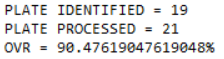
\includegraphics[width=6cm]{images/OVRKombinasiParameter.png}}
		\captionof{figure}{Hasil OVR Pengujian Kombinasi Parameter Gabungan\\}
		\label{fig:HasilOVRKombinasiParameterGabungan}
	\end{minipage}
\end{adjustbox}

\begin{adjustbox}{width=1\textwidth}
	\noindent\begin{minipage}{\linewidth}
		\centering\framebox{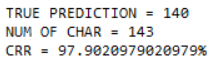
\includegraphics[width=6cm]{images/CRRKombinasiParameter.png}}
		\captionof{figure}{Hasil CRR Pengujian Kombinasi Parameter Gabungan\\}
		\label{fig:HasilCRRKombinasiParameterGabungan}
	\end{minipage}
\end{adjustbox}

\noindent Dari Gambar \ref{fig:HasilCRRKombinasiParameterGabungan} \textit{Character Recognition Rate} yang didapatkan adalah sebesar 97.90\%. Tingkat akurasi \textit{Character Recognition Rate} (CRR) meningkat 2\% terhadap hasil CRR kombinasi parameter dengan ukuran sel 8 $\times$ 8 piksel, jumlah \textit{bin} 18, dan nilai sigma 0.1. Dari 143 karakter yang terdeteksi, sebanyak 140 di antaranya dapat diklasifikasikan dengan baik, hal ini juga meningkatkan jumlah plat nomor yang berhasil dikenali. Sedangkan berdasarkan hasil OVR pada Gambar \ref{fig:HasilOVRKombinasiParameterGabungan} dari 21 plat nomor yang terdeteksi 19 plat nomor dapat dikenali dengan baik.\\

\section{Analisis Pengujian}
\noindent Setiap skenario pengujian yang dilakukan pada subbab 4.3.1 dan 4.3.2 diukur dengan melihat tingkat akurasi ada \textit{Character Recognition Rate} dan \textit{Overall Performance} yang mengukur performa keseluruhan aplikasi. Berdasarkan hasil pengujian pada Gambar \ref{fig:HasilPengujianUkuranSel2} sampai Gambar \ref{fig:HasilPengujianUkuranSel16}, tingginya tingkat akurasi OVR sangat bergantung kepada tingginya tingkat akurasi CRR, semakin tinggi tingkat akurasi dari CRR maka tingkat akurasi dari OVR juga akan semakin meningkat. Pada beberapa hasil pengujian terlihat juga OVR menunjukkan angka 0\%, hal ini disertai dengan rendahnya tingkat akurasi dari CRR pada hasil pengujian tersebut (biasanya terjadi ketika angka CRR berada di bawah 51\%). Hal ini disebabkan karena OVR menghitung jumlah plat yang dikenali dengan benar terhadap jumlah keseluruhan plat yang terdeteksi oleh sistem. Kondisi plat disebut dikenali dengan benar adalah ketika keseluruhan hasil prediksi karakter untuk plat tersebut sama persis dengan karakter asli pada citra plat, satu saja hasil prediksi karakter yang tidak sama akan membuat plat tersebut tidak dapat dimasukkan ke dalam kategori plat yang dapat dikenali dengan benar. Oleh karena itu, jika aplikasi tidak dapat mengenali setiap karakter dengan baik (angka akurasi CRR rendah) maka nilai OVR yang didapat pun akan rendah dan bahkan 0.

\noindent Tingkat akurasi CRR yang didapatkan bergantung terhadap komposisi parameter yang digunakan. Berdasarkan hasil CRR hasil pengujian pada Gambar \ref{fig:HasilPengujianUkuranSel2} sampai Gambar \ref{fig:HasilPengujianUkuranSel16} tingkat akurasi CRR optimal yang didapatkan cenderung meningkat ketika menggunakan kombinasi parameter dengan ukuran sel 2 $\times$ 2 piksel sampai dengan 8 $\times$ 8 piksel. Namun ketika menggunakan kombinasi parameter dengan ukuran sel 16 $\times$ 16 piksel, tingkat akurasi CRR optimal yang didapatkan menurun. Dari pola tersebut dapat disimpulkan untuk menghasilkan tingkat CRR yang optimal diperlukan komposisi parameter yang tepat.

\noindent Untuk nilai sigma pada metode \textit{SVM} yang digunakan agar tingkat akurasi CRR yang dihasilkan optimal, kecenderungan yang didapatkan dari hasil pengujian pada Gambar \ref{fig:HasilPengujianUkuranSel2} sampai Gambar \ref{fig:HasilPengujianUkuranSel16} adalah cenderung mengikuti besarnya ukuran sel, semakin ukuran selnya besar, maka semakin tinggi nilai sigma yang dibutuhkan.

\noindent Kombinasi parameter terbaik untuk setiap karakter dapat ditentukan dengan melihat hasil klasifikasi dari setiap hasil pengujian kombinasi parameter, yaitu pada tabel \ref{tab:hasilklasifikasisel2} sampai dengan tabel \ref{tab:hasilklasifikasisel16}. Dari tabel-tabel tersebut didapati bahwa kombinasi parameter dengan ukuran sel 8 $\times$ 8 piksel dapat mengklasifikasikan mayoritas karakter dengan baik terkecuali huruf Q dan huruf D. Kedua huruf tersebut memiliki akurasi klasifikasi yang paling baik ketika diuji menggunakan kombinasi parameter dengan ukuran 2 $\times$ 2 piksel, jumlah \textit{bin} 4, dan nilai sigma sebesar 0.01. Untuk huruf Q, ketika ia diuji menggunakan kombinasi parameter selain dengan ukuran sel 2 $\times$ 2 piksel, maka huruf tersebut akan selalu tertukar dengan angka 0.

\begin{adjustbox}{width=1\textwidth}
	\noindent\begin{minipage}{\linewidth}
		\centering\framebox{
\includegraphics[width=2cm]{images/HurufQ.png}}
		\begin{center}
			(a)
		\end{center}
	\end{minipage}
\end{adjustbox}

\begin{adjustbox}{width=1\textwidth}
	\noindent\begin{minipage}{\linewidth}
		\centering\framebox{
\includegraphics[width=2cm]{images/Angka0.png}}
		\begin{center}
			(b)
		\end{center}
		\captionof{figure}{Contoh citra (a) Huruf Q (b) Angka 0\\}
		\label{fig:hurufQangka0}
	\end{minipage}
\end{adjustbox}

\noindent Dari Gambar \ref{fig:hurufQangka0} dapat terlihat bahwa karakteristik objek yang dimiliki huruf Q dengan angka 0 memang mirip sehingga ketika dilakukan ekstraksi fitur terhadap kedua karakter tersebut tidak menutup kemungkinan fitur yang dihasilkan mirip. Oleh karena itu penggunaan ukuran sel 2 $\times$ 2 piksel memang tepat jika digunakan untuk mengklasifikasikan huruf Q dikarenakan ukuran sel 2 $\times$ 2 piksel dapat menangkap detail dari objek huruf Q dengan lebih baik dibandingkan ukuran sel lainnya.

\noindent Untuk huruf D, dari keseluruhan citra huruf D yang terdeteksi sistem, terdapat 1 citra yang awalnya dapat diklasifikasi dengan benar ketika menggunakan ukuran sel 2 $\times$ piksel, namun menjadi misklasifikasi ketika menggunakan ukuran sel lain. Setelah dilakukan analisis lebih lanjut, satu citra yang misklasifikasi tersebut ternyata memiliki masalah pada hasil segmentasi karakternya. Hal itu juga disebabkan karena citra karakter berasalh dari citra plat yang bermasalah (citra plat miring dan tidak tersegmentasi horizontal dengan baik). Hal ini tentunya akan berdampak sangat besar terhadap hasil segmentasi vertikalnya. Citra plat hasil \textit{preprocessing} dan segmentasi dan citra karakter D yang misklasifikasi dapat dilihat pada Gambar \ref{fig:CitraPlatMisklasifikasiD} dan Gambar \ref{fig:CitraHasilSegmentasiD}.

\begin{adjustbox}{width=1\textwidth}
	\noindent\begin{minipage}{\linewidth}
		\centering\framebox{
\includegraphics[width=8cm]{images/D1192PS.png}}
		\captionof{figure}{Citra Plat asal karakter D yang misklasifikasi\\}
		\label{fig:CitraPlatMisklasifikasiD}
	\end{minipage}
\end{adjustbox}

\begin{adjustbox}{width=1\textwidth}
	\noindent\begin{minipage}{\linewidth}
		\centering\framebox{
\includegraphics[width=1cm]{images/DMisklasifikasi.png}}
		\captionof{figure}{Citra hasil segmentasi karakter huruf D\\}
		\label{fig:CitraHasilSegmentasiD}
	\end{minipage}
\end{adjustbox}\\

\noindent Untuk meningkatkan akurasi pengenalan huruf Q dan huruf D, digunakanlah dua kombinasi parameter seperti yang sudah disinggung pada subbab 4.3.2. Dan dari hasil pengujian yang didapatkan terbukti dapat meningkatkan akurasi pengenalan terhadap huruf Q dan huruf D. Dari hasil pengujian tersebut dapat disimpulkan bahwa kombinasi parameter yang berbeda dapat diterapkan pada sistem untuk mencapai hasil yang lebih optimal.\\

\section{Analisis Kesalahan}
\noindent Berdasarkan keseluruhan hasil skenario pengujian, didapatkan bahwa akurasi pengenalan karakter paling tinggi dihasilkan dari penggabungan kombinasi parameter yang paling optimal untuk setiap karakter. Namun berdasarkan tabel \ref{tab:hasilklasifikasiselCampuran}, terdapat tiga citra karakter yang mengalami misklasifikasi. Karakter-karakter tersebut adalah angka 1 sebanyak satu citra dan angka 2 sebanyak dua citra. Hasil misklasifikasi karakter-karakter tersebut dapat dilihat pada tabel \ref{tab:analisiskesalahan}

\begin{longtable}[c]{|r|r|r|}
	\caption{Hasil klasifikasi karakter yang misklasifikasi}
	\label{tab:analisiskesalahan}\\
	\hline
	No & Karakter & Hasil Klasifikasi \\ \hline
	\endfirsthead
	%
	\multicolumn{3}{c}%
	{{\bfseries Table \thetable\ continued from previous page}} \\
	\hline
	No & Karakter & Hasil Klasifikasi \\ \hline
	\endhead
	%
	1  & 1        & D                 \\ \hline
	2  & 2        & D                 \\ \hline
\end{longtable}
 
%\noindent Berdasarkan hasil pengujian, didapatkan bahwa komposisi parameter yang menghasilkan akurasi paling tinggi dihasilkan oleh komposisi parameter dengan ukuran sel 8 $\times$ 8 piksel dan akurasi paling rendah dihasilkan oleh komposisi parameter dengan ukuran sel 2 $\times$ 2 piksel. Namun meskipun menghasilkan akurasi yang tertinggi dan banyak karakter yang jika dibandingkan dengan hasil pengujian menggunakan ukuran sel 2 $\times$ 2 piksel akurasinya meningkat, masih terdapat juga karakter yang kenaikan akurasinya tidak terlalu signifikan, ada karakter yang akurasinya berkurang, dan bahkan ada karakter yang tadinya dapat diklasifikasi dengan baik dan malah menjadi tidak dapat diklasifikasi dengan benar sama sekali. Karakter-karakter tersebut adalah angka 2, huruf D, dan huruf Q. Penjelasan dari kejadian ini diilustrasikan pada tabel \ref{tab:analisiskesalahan}.
%\begin{longtable}[c]{|c|c|c|c|c|c|c|c|}
%	\caption{Perbandingan hasil akurasi karakter pada ukuran sel 2 dengan ukuran sel 8}
%	\label{tab:analisiskesalahan}\\
%	\hline
%	\multirow{2}{*}{No} & \multirow{2}{*}{Karakter} & \multicolumn{3}{c|}{Ukuran Sel 2} & \multicolumn{3}{c|}{Ukuran Sel 8} \\ \cline{3-8} 
%	&  & Benar & Salah & Akurasi & Benar & Salah & Akurasi \\ \hline
%	\endfirsthead
%	%
%	\multicolumn{8}{c}%
%	{{\bfseries Table \thetable\ continued from previous page}} \\
%	\hline
%	\multirow{2}{*}{No} & \multirow{2}{*}{Karakter} & \multicolumn{3}{c|}{Ukuran Sel 2} & \multicolumn{3}{c|}{Ukuran Sel 8} \\ \cline{3-8} 
%	&  & Benar & Salah & Akurasi & Benar & Salah & Akurasi \\ \hline
%	\endhead
%	%
%	1 & 2 & 6 & 3 & 66.67\% & 7 & 2 & 77.78\% \\ \hline
%	2 & D & 20 & 0 & 100\% & 19 & 1 & 95\% \\ \hline
%	3 & Q & 2 & 0 & 100\% & 0 & 2 & 0\% \\ \hline
%\end{longtable}
\noindent Seperti yang ditunjukkan pada tabel \ref{tab:analisiskesalahan}, keseluruhan angka 1 dan 2 yang misklasifikasi dianggap sebagai karakter huruf D. Kombinasi parameter yang digunakan untuk mengklasifikasikan karakter angka 1 dan angka 2 adalah kombinasi parameter yang paling optimal untuk kedua karakter tersebut berdasarkan hasil pengujian pada subbab 4.3.1, yaitu ukuran sel 8 $\times$ 8 piksel, jumlah \textit{bin} 18, dan nilai sigma 0.1. Setelah ditelusuri, ternyata karakter angka 1 dan satu dari dua angka 2 yang misklasifikasi berasal dari citra plat yang sama, yaitu citra plat pada Gambar \ref{fig:CitraPlatMisklasifikasiD}, sedangkan citra angka 2 yang satunya berasal dari citra plat seperti yang ditunjukkan pada Gambar \ref{fig:CitraPlatMisklasifikasi2}.

\begin{adjustbox}{width=1\textwidth}
	\noindent\begin{minipage}{\linewidth}
		\centering\framebox{
\includegraphics[width=8cm]{images/D1278LI.png}}
		\captionof{figure}{Citra Plat asal karakter angka 2 yang misklasifikasi\\}
		\label{fig:CitraPlatMisklasifikasi2}
	\end{minipage}
\end{adjustbox}

\noindent Pada gambar \ref{fig:CitraPlatMisklasifikasiD} dan Gambar \ref{fig:CitraPlatMisklasifikasi2}, dapat dilihat bahwa citra plat yang didapatkan tidak lurus dan tidak tersegmentasi horizontal dengan baik. Hal ini akan mempengaruhi hasil segmentasi vertikal ketika mencari area karakter dari plat tersebut. Hasil segmentasi untuk setiap karakter dapat dilihat pada Gambar \ref{fig:CitraHasilSegmentasiKarakterMisklasifikasi}.

\begin{adjustbox}{width=1\textwidth}
	\noindent\begin{minipage}{\linewidth}
		\centering\framebox{
\includegraphics[width=1cm]{images/1Misklasifikasi.png}}
		\begin{center}
			(a)
		\end{center}
	\end{minipage}
\end{adjustbox}

\begin{adjustbox}{width=1\textwidth}
	\noindent\begin{minipage}{\linewidth}
		\centering\framebox{
\includegraphics[width=1cm]{images/2Misklasifikasi1.png}}
		\begin{center}
			(b)
		\end{center}
	\end{minipage}
\end{adjustbox}

\begin{adjustbox}{width=1\textwidth}
	\noindent\begin{minipage}{\linewidth}
		\centering\framebox{
\includegraphics[width=1cm]{images/2Misklasifikasi2.png}}
		\begin{center}
			(c)
		\end{center}
		\captionof{figure}{Citra hasil segmentasi karakter misklasifikasi (a) Citra angka 1 dengan satu objek lain (b) Citra angka 2 dengan dua objek lain (c) Citra angka 2 dengan satu objek lain \\}
		\label{fig:CitraHasilSegmentasiKarakterMisklasifikasi}
	\end{minipage}
\end{adjustbox}

%\noindent Seperti yang ditunjukkan pada tabel \ref{tab:analisiskesalahan} di atas, angka 2 kenaikan akurasinya tidak begitu signifikan dikarenakan hanya berbeda 1 hasil klasifikasi yang benar, huruf D mengalami penurunan akurasi dikarenakan terdapat karakter yang tadinya dapat diklasifikasi dengan benar dan ketika ukuran sel diganti menjadi 8 $\times$ 8 piksel, karakter tersebut malah menjadi tidak terklasifikasi dengan benar. Sedangkan untuk huruf Q, awalnya karakter tersebut dapat dikenali dengan baik namun setelah menggunakan ukuran sel 8 $\times$ 8 piksel, karakter tersebut menjadi tidak dapat terklasifikasi dengan baik.
%\noindent Pada karakter angka 2, ketika dilihat pada hasil dari \textit{Confusion Matrix} ternyata ketika menggunakan ukuran sel 2 $\times$ 2 piksel, terdapat 3 karakter yang teridentifikasi sebagai karakter huruf D, dan ketika menggunakan ukuran sel 8 $\times$ 8 piksel berubah menjadi teridentifikasi sebagai karakter huruf O. Namun ada satu citra karakter angka 2 yang tadinya tidak dapat diklasifikasikan dengan benar ketika menggunakan ukuran sel 2 $\times$ 2 piksel dan menjadi dapat diklasifikan dengan benar ketika menggunakan ukuran sel 8 $\times$ 8 piksel. Gambar \ref{fig:CitraPlat} merupakan citra plat hasil \textit{preprocessing} dari karakter angka 2 tersebut.\\

%\begin{adjustbox}{width=1\textwidth}
%	\noindent\begin{minipage}{\linewidth}
%		\centering\framebox{
\includegraphics[width=8cm]{images/D1623RB.png}}
%		\captionof{figure}{Citra Plat\\}
%		\label{fig:CitraPlat}
%	\end{minipage}
%\end{adjustbox}\\
%\\
%\noindent Dari citra plat dapat dilihat bahwa tidak ada masalah dengan bentuk dari plat itu sendiri (tidak miring dan berhasil tersegmentasi secara horizontal dengan baik). Jadi apabila terdapat kesalahan klasifikasi hal tersebut dikarenakan dari fitur yang dihasilkan dari \textit{HOG} dengan ukuran sel 2 $\times$ 2 piksel tidak cukup baik dibandingkan dengan \textit{HOG} ukuran sel 8 $\times$ 8 piksel. Sedangkan untuk 2 citra karakter angka 2 yang tetap tidak dapat diklasifikasikan dengan baik, berikut adalah citra plat tempat citra karakter berasal.\\
%
%\noindent Dari citra dapat dilihat bahwa kedua citra karakter angka 2 yang misklasifikasi tersebut berasal dari citra plat yang bermasalah (citra plat miring dan tidak tersegmentasi horizontal dengan baik). Hal ini tentunya akan berdampak sangat besar kepada hasil segmentasi vertikalnya. Berikut adalah hasil segmentasi vertikal angka 2 dari kedua plat tersebut.\\\\
%\begin{adjustbox}{width=1\textwidth}
%	\noindent\begin{minipage}{\linewidth}
%		\centering\framebox{
\includegraphics[width=1cm]{images/2Misklasifikasi1.png}}
%		\begin{center}
%			(a)
%		\end{center}
%	\end{minipage}
%\end{adjustbox}\\\\\\
%\begin{adjustbox}{width=1\textwidth}
%	\noindent\begin{minipage}{\linewidth}
%		\centering\framebox{
\includegraphics[width=1cm]{images/2Misklasifikasi2.png}}
%		\begin{center}
%			(b)
%		\end{center}
%		\captionof{figure}{Citra hasil segmentasi karakter angka 2, (a) citra dengan tiga objek di dalamnya (b) citra dengan dua objek di dalamnya\\}
%		\label{fig:CitraHasilSegmentasi2}
%	\end{minipage}
%\end{adjustbox}\\
%\\
\noindent Dari citra hasil segmentasi pada Gambar \ref{fig:CitraHasilSegmentasiKarakterMisklasifikasi} dapat dilihat bahwa terdapat objek lain selain objek utama pada hasil segmentasi vertikal ketiga citra karakter angka 1 dan citra karakter angka 2 yang misklasifikasi. Hal ini akan berdampak pada hasil fitur yang akan dihasilkan dari metode \textit{HOG} nantinya. Oleh karena itu, bisa disimpulkan kondisi citra plat yang kurang baik yang menyebabkan kedua karakter ini tidak dapat diidentifikasi.

%\noindent Pada tabel \ref{tab:analisiskesalahan} juga dapat dilihat terdapat satu citra karakter D yang awalnya dapat diklasifikasi dengan baik ketika menggunakan ukuran sel 2 $\times$ 2 piksel namun menjadi misklasifikasi ketika menggunakan ukuran sel 8 $\times$ 8 piksel. Setelah melihat hasil klasifikasi pada tabel \textit{Confusion Matrix} ternyata karakter D tersebut teridentifikasi sebagai karakter huruf O. Dan setelah ditelusuri, ternyata citra karakter huruf D tersebut berasal dari citra plat yang sama dengan citra plat yang menyebabkan 2 citra karakter angka 2 misklasfikasi, yaitu citra plat D1192PS seperti yang pernah ditampilkan sebelumnya (Gambar \ref{fig:CitraPlatMisklasifikasi} atas). Adapun hasil segmentasi vertikal dari karakter huruf D tersebut dapat dilihat pada Gambar \ref{fig:CitraHasilSegmentasiD}.
%
%\noindent Dari citra dapat dilihat bahwa terdapat objek garis yang merupakan garis tepi dari plat nomor. Hal inilah yang akan berdampak pada hasil fitur yang akan dihasilkan dari metode \textit{HOG} nantinya. Untuk kasus ini, citra karakter ini bisa diklasifikasikan sebagai karakter huruf D ketika menggunakan ukuran sel 2 $\times$ 2 piksel dan tidak dapat diklasifikan dengan benar ketika menggunakan ukuran sel 8 $\times$ 8 piksel sehingga bisa diasumsikan bahwa peranan ukuran sel berpengaruh dalam hasil klasifikasi, secara teori ukuran sel yang lebih kecil memang memiliki kelebihan untuk menangkap detil yang lebih baik jika dibandingkan dengan ukuran sel yang besar, walaupun dengan demikian ukuran fitur yang dihasilkan oleh ukuran sel yang kecil akan jauh lebih besar dibandingkan fitur dari ukuran sel yang lebih besar.
%
%\noindent Asumsi di atas didukung dengan melihat data berikutnya pada tabel \ref{tab:analisiskesalahan}. Terdapat karakter huruf Q yang ketika menggunakan ukuran sel 2 $\times$ 2 piksel dapat diklasifikasikan dengan baik tetapi ketika menggunakan ukuran sel 8 $\times$ 8 piksel malah terjadi misklasifikasi. Jika dilihat pada tabel hasil klasifikasi dengan ukuran sel di atas 2, memang karakter huruf Q tersebut sudah tidak dapat diklasifikasi dengan benar lagi dan selalu tertukar dengan karakter angka 0.
%
%\noindent Dari hasil analisis kesalahan ini dapat disimpulkan beberapa faktor yang berpengaruh terhadap hasil fitur dari \textit{HOG} yang nantinya juga akan berpengaruh terhadap akurasi dari klasifikasi karakter menggunakan SVM, yaitu faktor eksternal seperti masalah pada citra yang kurang baik (citra plat miring) dan faktor internal seperti ukuran sel dan jika diamati dari hasil pengujian jumlah bin cenderung mengikuti ukuran sel, semakin besar ukuran sel maka untuk menghasilkan akurasi yang maksimal pada ukuran sel tersebut diperlukan jumlah bin yang lebih besar juga, begitu pun dengan nilai sigma yang digunakan untuk metode \textit{Support Vector Machine} sebagai metode klasifikasinya.
\newpage